% Курсова робота з освітнього компоненту «Моделювання систем. Курсова робота», завдання В12.
% Структура — за посібником Стеценко І. В. та ін. (2024): титул (додаток А), завдання (додаток Б),
% анотація (додаток В), зміст, вступ, п'ять розділів, висновки, джерела, додатки.
\documentclass[coursework]{kpi-thesis}
\usepackage{kpi-titles}
\usepackage{fvextra}
\usepackage{tikz}
\usetikzlibrary{arrows.meta,positioning,shapes.multipart,shapes.geometric,calc,fit}

% Посібник вимагає полів 2 см з усіх боків.
\geometry{left=20mm,right=20mm,top=20mm,bottom=20mm}
\graphicspath{{media/}{../model/out/}}

\kpiset{
  title      = {Імітаційна модель системи посадки літаків в аеропорту на основі формального опису стохастичною мережею Петрі},
  discipline = {Моделювання систем. Курсова робота},
  group      = {ІП-34},
  gender     = {m},
  student    = {Микола ТУБОЛЕВ},
  advisor    = {ас. Коринецький Д. С.},
  year       = {2026},
}
\newcommand\recordbook{№ 14309039}
% Члени комісії на титулі — у форматі «Ім'я ПРІЗВИЩЕ».
\newcommand\advisorCommission{Д. КОРИНЕЦЬКИЙ}

% Код моделі з українськими коментарями: listings під XeLaTeX псує розділові знаки поряд з кирилицею.
\fvset{fontsize=\setstretch{1}\fontsize{10}{11.5}\selectfont, breaklines, breakanywhere, tabsize=2, xleftmargin=1.25cm}
\newcommand\tsfile[1]{%
  \par\noindent\textbf{Файл }\path{#1}\par
  \VerbatimInput[fontsize=\setstretch{1}\fontsize{9}{10.5}\selectfont, xleftmargin=0pt]{../model/#1}%
}
\newcommand\code[1]{\texttt{#1}}
\newcolumntype{L}[1]{>{\raggedright\arraybackslash}p{#1}}

\kpiloadstats{self}{build/main.kpistats}

\makeatletter
\newcommand\courseworkTitle{%
  \begingroup
  \thispagestyle{empty}%
  \setstretch{1.15}%
  \begin{center}
  МІНІСТЕРСТВО ОСВІТИ І НАУКИ УКРАЇНИ\\
  НАЦІОНАЛЬНИЙ ТЕХНІЧНИЙ УНІВЕРСИТЕТ УКРАЇНИ\\
  «КИЇВСЬКИЙ ПОЛІТЕХНІЧНИЙ ІНСТИТУТ імені ІГОРЯ СІКОРСЬКОГО»\\
  КАФЕДРА ІНФОРМАТИКИ ТА ПРОГРАМНОЇ ІНЖЕНЕРІЇ

  \vspace{3.5cm}
  Курсова робота з освітнього компоненту\\
  «\kpi@g{discipline}»

  \vspace{0.3cm}
  Тема: \textbf{\kpi@g{title}}
  \end{center}

  \vspace{2.5cm}
  \noindent
  \begin{minipage}[t]{0.47\textwidth}
  \raggedright
  Керівник:\\
  \kpi@g{advisor}

  \vspace{0.6cm}
  «Допущено до захисту»\\
  \sigline{5cm}

  «\sigline{0.8cm}» \sigline{3cm} 20\sigline{0.6cm} р.

  \vspace{0.6cm}
  Захищено з оцінкою\\
  \sigline{5cm}
  \end{minipage}%
  \hfill
  \begin{minipage}[t]{0.47\textwidth}
  \raggedright
  Виконавець:\\
  \kpi@g{student}\\
  студент групи \kpi@g{group}\\
  залікова книжка \recordbook

  \vspace{0.6cm}
  \sigline{5cm}

  «\sigline{0.8cm}» \sigline{3cm} 20\sigline{0.6cm} р.
  \end{minipage}

  \vspace{1cm}
  \noindent Члени комісії:

  \vspace{0.3cm}
  \noindent\sigline{5cm}\hfill\makebox[0.47\textwidth][l]{Інна СТЕЦЕНКО}

  \vspace{0.4cm}
  \noindent\sigline{5cm}\hfill\makebox[0.47\textwidth][l]{\advisorCommission}

  \vfill
  \begin{center}
  Київ -- \kpi@g{year}
  \end{center}
  \endgroup
  \clearpage
}
\makeatother

\begin{document}
\courseworkTitle
\mainmatter

\structural{ЗАВДАННЯ}

Виконати дослідження для такої системи.

Потік літаків, що потребують посадки в аеропорті, пуассонівський з інтенсивністю 10~літаків за годину. В аеропорту є дві посадкові смуги. Літак, зробивши посадку на смугу, звільняє її через 35~хвилин. Якщо літак потребує посадки, коли усі смуги зайняті, він очікує на посадку. Якщо очікування на посадку триває більше ніж $70 \pm 10$~хвилин, то виникає необхідність дозаправки літака, на що аеропорту доведеться витратити $1000 \pm 200$~грошових одиниць. Після 140~хвилин очікування літак відправляється на посадку в інший аеропорт. За кожний літак, що здійснив посадку без очікування, аеропорт має прибуток 2000~гривень, а за кожний, що здійснив посадку з очікуванням, -- $1500 \pm 100$~гривень. Витрати на будівництво додаткової посадкової смуги складають 3\,000\,000~гривень. В аеропорту не може бути побудовано більше ніж 10~додаткових смуг.

Метою моделювання є визначення кількості посадкових смуг, при якій інтервал часу їх окупності буде мінімальним, якщо час окупності додаткових посадкових смуг складає
\[
T = \frac{S}{p},
\]
де $S$ -- витрати на побудову смуг, $p$ -- прибуток за один рік.

Для вищезазначеної системи:
\begin{enumerate}[label=\arabic*)]
\item розробити опис концептуальної моделі системи;
\item виконати формалізацію опису об'єкта моделювання в термінах стохастичної мережі Петрі;
\item розробити алгоритм імітації моделі дискретно-подійної системи у відповідності до побудованого формального опису;
\item для доведення коректності побудованого алгоритму виконати верифікацію алгоритму імітації;
\item визначити статистичні оцінки заданих характеристик моделі, що є метою моделювання;
\item провести експериментальне дослідження моделі;
\item інтерпретувати результати моделювання та сформулювати пропозиції щодо поліпшення функціонування системи;
\item зробити висновки щодо складності розробки моделі та алгоритму імітації на основі використаного формалізму, отриманих результатів моделювання та їх корисності.
\end{enumerate}

\structural{АНОТАЦІЯ}

Туболев М. Курсова робота на тему «Імітаційна модель системи посадки літаків в аеропорту на основі формального опису стохастичною мережею Петрі».

Текстова частина курсової роботи складається із вступу, п'яти розділів, висновків, списку використаних джерел з \kpistatof{self}{sources} найменувань та \kpistatof{self}{appendices} додатків, які викладено на \kpistatof{self}{pages} сторінках. В тексті роботи оформлено \kpistatof{self}{figures} рисунків, \kpistatof{self}{tables} таблиць.

У роботі поставлено завдання визначити кількість посадкових смуг аеропорту, за якої час окупності додаткових смуг мінімальний. Літаки надходять пуассонівським потоком, займають смугу на 35~хвилин, за тривалого очікування потребують дозаправки, а після 140~хвилин відлітають в інший аеропорт.

Імітаційна модель розроблена на основі формального опису стохастичною мережею Петрі з часовими затримками, у якій кожен літак представлено окремим маркером-об'єктом. Це дозволило точно відтворити індивідуальні таймери дозаправки й відльоту кожного літака. Алгоритм імітації мережі Петрі реалізовано мовою TypeScript у середовищі виконання Bun без бібліотек імітаційного моделювання. Коректність алгоритму підтверджено модульними тестами та верифікацією моделі за вісьмома наборами вхідних даних.

Проведено дослідження перехідного періоду, визначено тривалість прогону (рік модельного часу після доби розгону) і кількість повторних прогонів (51) для довірчої ймовірності 0,95. Повним перебором досліджено від 0 до 10 додаткових смуг.

Результати моделювання свідчать, що за двох смуг аеропорт збитковий: майже кожен літак дозаправляється, дві третини літаків відлітають. Найменший час окупності, близько 0,93~місяця, досягається за семи смуг, тобто за п'яти додаткових; за них жоден літак не відлітає, а середнє очікування скорочується до 9~хвилин.

Зроблено висновок, що аеропорту доцільно збудувати п'ять додаткових смуг. Пробний запуск за інтенсивності 8 і 12~літаків на годину показав, що оптимум зсувається до 5 і 8~смуг відповідно, тож за очікуваного зростання потоку варто передбачити шосту додаткову смугу.

Ключові слова: імітаційна модель, алгоритм імітації, стохастична мережа Петрі, аеропорт, час окупності, TypeScript.

\tableofcontents
\structural{ВСТУП}

Аеропорт із недостатньою кількістю посадкових смуг втрачає гроші двома шляхами: літаки, що довго чекають посадки, доводиться дозаправляти, а частина літаків, не дочекавшись, відлітає в інші аеропорти. Будівництво нових смуг усуває ці втрати, але коштує значних грошей, і кожна наступна смуга дає менший приріст прибутку, ніж попередня. Тому питання, скільки смуг збудувати, має кількісну відповідь: таку кількість, за якої вкладені кошти повертаються найшвидше.

Аналітично цю задачу розв'язати важко. Надходження літаків випадкові, кожен літак має власні таймери дозаправки й відльоту, що відраховуються від моменту його прибуття, а дохід і витрати залежать від того, як довго чекав саме цей літак. Класичні формули теорії масового обслуговування не враховують одночасно нетерплячих клієнтів з двома порогами очікування й вартісні показники. Імітаційне моделювання дозволяє відтворити процес функціонування системи в часі й отримати статистичні оцінки потрібних показників без спрощувальних припущень~\cite{stetsenko2010, tomashevskyi2005}.

\textbf{Тема роботи} -- імітаційна модель системи посадки літаків в аеропорту на основі формального опису стохастичною мережею Петрі.

\textbf{Мета роботи} -- визначити кількість посадкових смуг, за якої час окупності додаткових смуг $T = S/p$ мінімальний, де $S$ -- витрати на будівництво смуг, $p$ -- річний прибуток.

Для досягнення мети потрібно:
\begin{itemize}
\item описати концептуальну модель системи: процес, вхідні та вихідні змінні;
\item побудувати формальний опис моделі стохастичною мережею Петрі й визначити формули вихідних характеристик;
\item розробити й реалізувати алгоритм імітації мережі Петрі та верифікувати модель;
\item визначити тривалість перехідного періоду, тривалість прогону і кількість повторних прогонів;
\item провести експериментальне дослідження для 0--10 додаткових смуг, знайти оптимальну кількість і сформулювати пропозиції.
\end{itemize}

Роботу виконано за рекомендаціями посібника~\cite{stetsenko2024}. Формалізмом опису обрано стохастичну мережу Петрі з часовими затримками. Літаки в моделі представлено маркерами-об'єктами з ідентифікатором і моментом прибуття, що близько до ідеї кольорових мереж Петрі~\cite{jensen2009}: так кожен літак отримує власні таймери, а мережа лишається компактною.

Модель і алгоритм імітації реалізовано мовою TypeScript~\cite{typescript} у середовищі виконання Bun~\cite{bun} без сторонніх бібліотек імітаційного моделювання. Програма будує схему мережі з того самого опису, що й модель, проводить усі експерименти й будує графіки для звіту.

\section{Концептуальна модель системи}

\subsection{Опис системи та процесу її функціонування}

Система, що моделюється, -- аеропорт, який приймає літаки на посадку. У ній можна виділити чотири підсистеми:
\begin{itemize}
\item \textbf{потік літаків} -- літаки, що потребують посадки, прибувають у випадкові моменти часу, у середньому 10~літаків за годину;
\item \textbf{посадкові смуги} -- $n$~однакових смуг; літак, що сів на смугу, звільняє її через 35~хвилин;
\item \textbf{черга очікування} -- літаки, які прибули, коли всі смуги зайняті, кружляють над аеропортом і чекають на посадку;
\item \textbf{фінансова підсистема} -- аеропорт отримує дохід за кожну посадку, сплачує за дозаправку літаків, що довго чекають, і вкладає кошти в будівництво додаткових смуг.
\end{itemize}

Процес обслуговування одного літака показано на рисунку~\ref{fig:process}. Якщо в момент прибуття є вільна смуга, літак одразу сідає, і аеропорт отримує 2000~грн. Інакше літак стає в чергу. З моменту прибуття для нього відраховуються два інтервали. Перший -- поріг дозаправки, від 60 до 80~хвилин: якщо літак досі не сів, аеропорт дозаправляє його, витрачаючи від 800 до 1200~грн. Другий -- 140~хвилин: якщо літак за цей час не сів, він відлітає в інший аеропорт, і аеропорт нічого за нього не отримує. Літак, що дочекався вільної смуги, сідає й приносить від 1400 до 1600~грн.

\begin{figure}[H]
\centering
\begin{tikzpicture}[
  font=\fontsize{11}{13}\selectfont,
  node distance=0.7cm and 1.0cm,
  box/.style={draw, rounded corners=2pt, align=center, minimum height=1.0cm, text width=3.9cm},
  money/.style={box, fill=gray!12},
  cond/.style={draw, diamond, aspect=2.4, align=center, inner sep=1pt, text width=2.9cm},
  arr/.style={-{Stealth[length=2.2mm]}},
]
\node[box] (arrive) {Прибуття літака\\(у середньому 10 за год)};
\node[cond, below=of arrive] (free) {Є вільна\\смуга?};
\node[money, right=1.6cm of free] (now) {Посадка без очікування\\дохід 2000 грн};
\node[box, below=of free] (queue) {Очікування в черзі};
\node[cond, below=of queue] (got) {Смуга звільнилась\\до 140 хв?};
\node[money, right=1.6cm of got] (late) {Посадка з очікуванням\\дохід $1500 \pm 100$ грн};
\node[box, below=of got] (leave) {Відліт в інший аеропорт\\дохід 0 грн};
\node[money, left=1.2cm of queue] (fuel) {Дозаправка, якщо чекає\\довше $70 \pm 10$ хв\\витрати $1000 \pm 200$ грн};
\node[box] (busy) at (now |- queue) {Смуга зайнята 35 хв,\\потім вільна};
\draw[arr] (arrive) -- (free);
\draw[arr] (free) -- node[above]{так} (now);
\draw[arr] (free) -- node[right]{ні} (queue);
\draw[arr] (queue) -- (got);
\draw[arr] (got) -- node[above]{так} (late);
\draw[arr] (got) -- node[right]{ні} (leave);
\draw[arr, dashed] (queue) -- (fuel);
\draw[arr] (now) -- (busy);
\draw[arr] (late) -- (busy);
\end{tikzpicture}
\caption{Процес обслуговування літака в аеропорту}
\label{fig:process}
\end{figure}

Літаки в черзі сідають у порядку прибуття. Коли смуга звільняється, першим сідає літак, що чекає найдовше, а не той, що прибув саме в цей момент. Дозаправка не зупиняє відлік до відльоту: дозаправлений літак, що так і не дочекався смуги, через 140~хвилин після прибуття все одно відлітає, і витрати на його дозаправку аеропорт уже поніс.

Аеропорт може збудувати від 0 до 10~додаткових смуг, кожна коштує 3\,000\,000~грн. Додаткові смуги прискорюють посадку, скорочують чергу, кількість дозаправок і відльотів, а отже підвищують річний прибуток. Час окупності $T = S/p$ показує, за скільки часу цей приріст прибутку поверне витрати $S$ на будівництво. Метою моделювання є кількість смуг, за якої $T$ мінімальний.

\subsection{Припущення моделі}

Текст завдання залишає кілька моментів невизначеними. У моделі прийнято такі припущення:
\begin{itemize}
\item запис «$70 \pm 10$ хвилин» означає, що поріг дозаправки кожного літака -- рівномірно розподілена величина на $[60; 80]$~хв; так само дохід $1500 \pm 100$~грн і витрати $1000 \pm 200$~грн рівномірно розподілені на $[1400; 1600]$ і $[800; 1200]$~грн;
\item літак дозаправляється не більше одного разу, а поріг дозаправки (не більше 80~хв) завжди менший за час відльоту (140~хв);
\item смуга зайнята 35~хвилин незалежно від того, чекав літак чи ні; смуги не відмовляють і однакові;
\item черга не обмежена за довжиною, літаки в ній обслуговуються в порядку прибуття;
\item у прибуток $p$ входять лише дохід від посадок і витрати на дозаправку, перераховані на 365~діб; інших витрат аеропорту в завданні немає;
\item $S$ -- витрати лише на додаткові смуги, тобто $S = 3 \cdot 10^6 \cdot k$~грн за $k$ додаткових смуг.
\end{itemize}

Прибуток $p$ у формулі окупності можна розуміти двояко. Окупність інвестицій зазвичай рахують за тим прибутком, який ці інвестиції приносять, тобто за приростом річного прибутку порівняно з аеропортом без нових смуг. У роботі це основна інтерпретація. Друга -- загальний річний прибуток аеропорту з новими смугами; за двох смуг він від'ємний, тож вона має сенс лише за достатньої кількості смуг. Модель обчислює обидва варіанти, а розділ~\ref{sec:experiment} показує, що оптимум за ними однаковий.

\subsection{Вхідні змінні моделі}

Вхідні змінні та параметри моделі наведено в таблиці~\ref{tab:inputs}. Керованою змінною є лише кількість посадкових смуг~$n$; решта параметрів задані умовою завдання.

\begin{kpitable}{|L{5.6cm}|L{2.7cm}|L{4.1cm}|L{3.0cm}|}{Вхідні змінні моделі\label{tab:inputs}}{\textbf{Змінна} & \textbf{Позначення} & \textbf{Значення} & \textbf{Одиниці}}
Кількість посадкових смуг (керована) & $n$ & $2 + k$, $k = 0, \ldots, 10$ & смуг \\ \hline
Інтенсивність надходження літаків & $\lambda$ & 10, експоненційні інтервали із середнім 6~хв & літаків / год \\ \hline
Час зайнятості смуги після посадки & $t_s$ & 35 & хв \\ \hline
Поріг очікування до дозаправки & $t_r$ & рівномірно на $[60; 80]$ & хв \\ \hline
Час очікування до відльоту & $t_l$ & 140 & хв \\ \hline
Дохід за посадку без очікування & $c_0$ & 2000 & грн \\ \hline
Дохід за посадку з очікуванням & $c_1$ & рівномірно на $[1400; 1600]$ & грн \\ \hline
Витрати на дозаправку & $z$ & рівномірно на $[800; 1200]$ & грн \\ \hline
Вартість однієї додаткової смуги & $s$ & 3\,000\,000 & грн \\ \hline
Найбільша кількість додаткових смуг & $k_{\max}$ & 10 & смуг \\ \hline
\end{kpitable}

\subsection{Вихідні змінні моделі}

Вихідні змінні наведено в таблиці~\ref{tab:outputs}. Цільовою характеристикою є час окупності $T$; решта пояснюють, звідки береться прибуток, і потрібні для верифікації моделі.

\begin{kpitable}{|L{7.0cm}|L{2.7cm}|L{5.7cm}|}{Вихідні змінні моделі\label{tab:outputs}}{\textbf{Змінна} & \textbf{Позначення} & \textbf{Одиниці}}
Кількість літаків, що прибули & $N_a$ & літаків \\ \hline
Кількість посадок без очікування & $N_0$ & літаків \\ \hline
Кількість посадок з очікуванням & $N_1$ & літаків \\ \hline
Кількість дозаправок & $N_r$ & літаків \\ \hline
Кількість літаків, що відлетіли в інший аеропорт & $N_l$ & літаків \\ \hline
Середній час очікування посадки & $W$ & хв \\ \hline
Середня та найбільша довжина черги & $L$, $L_{\max}$ & літаків \\ \hline
Середня кількість зайнятих смуг & $B$ & смуг \\ \hline
Дохід від посадок і витрати на дозаправку & $D$, $C$ & грн \\ \hline
Річний прибуток аеропорту & $P$ & грн / рік \\ \hline
Приріст річного прибутку порівняно з $n = 2$ & $\Delta P$ & грн / рік \\ \hline
Час окупності додаткових смуг & $T$ & місяців \\ \hline
\end{kpitable}

\subsection{Висновки до розділу}

Аеропорт описано як систему з потоком літаків, $n$~посадковими смугами, чергою очікування і фінансовою підсистемою. Особливість системи -- нетерплячі літаки з двома індивідуальними порогами очікування: після $70 \pm 10$~хв літак дозаправляють, після 140~хв він відлітає. Визначено вхідні змінні (керована -- кількість смуг $n$ від 2 до 12) і вихідні змінні, серед яких цільова -- час окупності додаткових смуг $T$. Сформульовано припущення, що уточнюють текст завдання.

\section{Формалізована модель системи}

\subsection{Елементи формалізму}

Модель описано стохастичною мережею Петрі з часовими затримками~\cite{stetsenko2010, stetsenko2024}. Позиція відтворює умову, кількість маркерів у ній -- кількість об'єктів, для яких умова виконана. Перехід відтворює подію і має три параметри: часову затримку $d$, пріоритет $r$ (за замовчуванням 0, більше значення -- вищий пріоритет) та ймовірність запуску $b$ (за замовчуванням 1). Вхідні дуги задають умову запуску переходу, вихідні -- наслідки події. Інформаційна дуга перевіряє наявність маркерів у позиції, але не забирає їх. Переходи багатоканальні: якщо умова запуску виконана кілька разів, перехід одночасно обслуговує кілька маркерів, кожен зі своїм моментом виходу. Затримки позначено так, як у посібнику~\cite{stetsenko2024}: $\exp(d)$ -- експоненційний закон із середнім $d$, $\mathrm{unif}(d; s)$ -- рівномірний закон на інтервалі $[d - s; d + s]$, число -- стала затримка.

Звичайна мережа Петрі не розрізняє маркери в позиції. Для цієї задачі цього недостатньо: кожен літак має власні таймери дозаправки й відльоту, і коли таймер спрацьовує, треба перевірити, чи в черзі ще є \emph{саме цей} літак. Якщо маркери безіменні, таймер одного літака забрав би з черги інший літак. Тому мережу доповнено маркерами-об'єктами, як у кольорових мережах Петрі~\cite{jensen2009}, але в мінімальному обсязі:
\begin{itemize}
\item \textbf{маркер-об'єкт} має номер і момент створення; його створює перехід-генератор (позначка \code{spawn});
\item \textbf{дуга з позначкою match} (вхідна або інформаційна) бере з позиції маркер того самого об'єкта, що й інші дуги match цього переходу; якщо таких дуг кілька, перехід запускається лише для об'єкта, присутнього в усіх відповідних позиціях; об'єкт шукається в порядку надходження в першій такій позиції;
\item \textbf{дуга з позначкою carry} кладе у вихідну позицію той самий об'єкт, що пройшов перехід, а не безіменний маркер.
\end{itemize}
Решта правил -- такі самі, як у стохастичній мережі Петрі: конфлікт переходів розв'язується спершу за пріоритетом, потім за ймовірністю запуску.

\subsection{Схема мережі Петрі}

Мережу Петрі, що формально описує аеропорт, наведено на рисунку~\ref{fig:petri}. Під назвою переходу вказано затримку й пріоритет, якщо він не нульовий; штрихова лінія -- інформаційна дуга. Позиції наведено в таблиці~\ref{tab:places}, переходи -- у таблиці~\ref{tab:transitions}.

\begin{figure}[H]
\centering
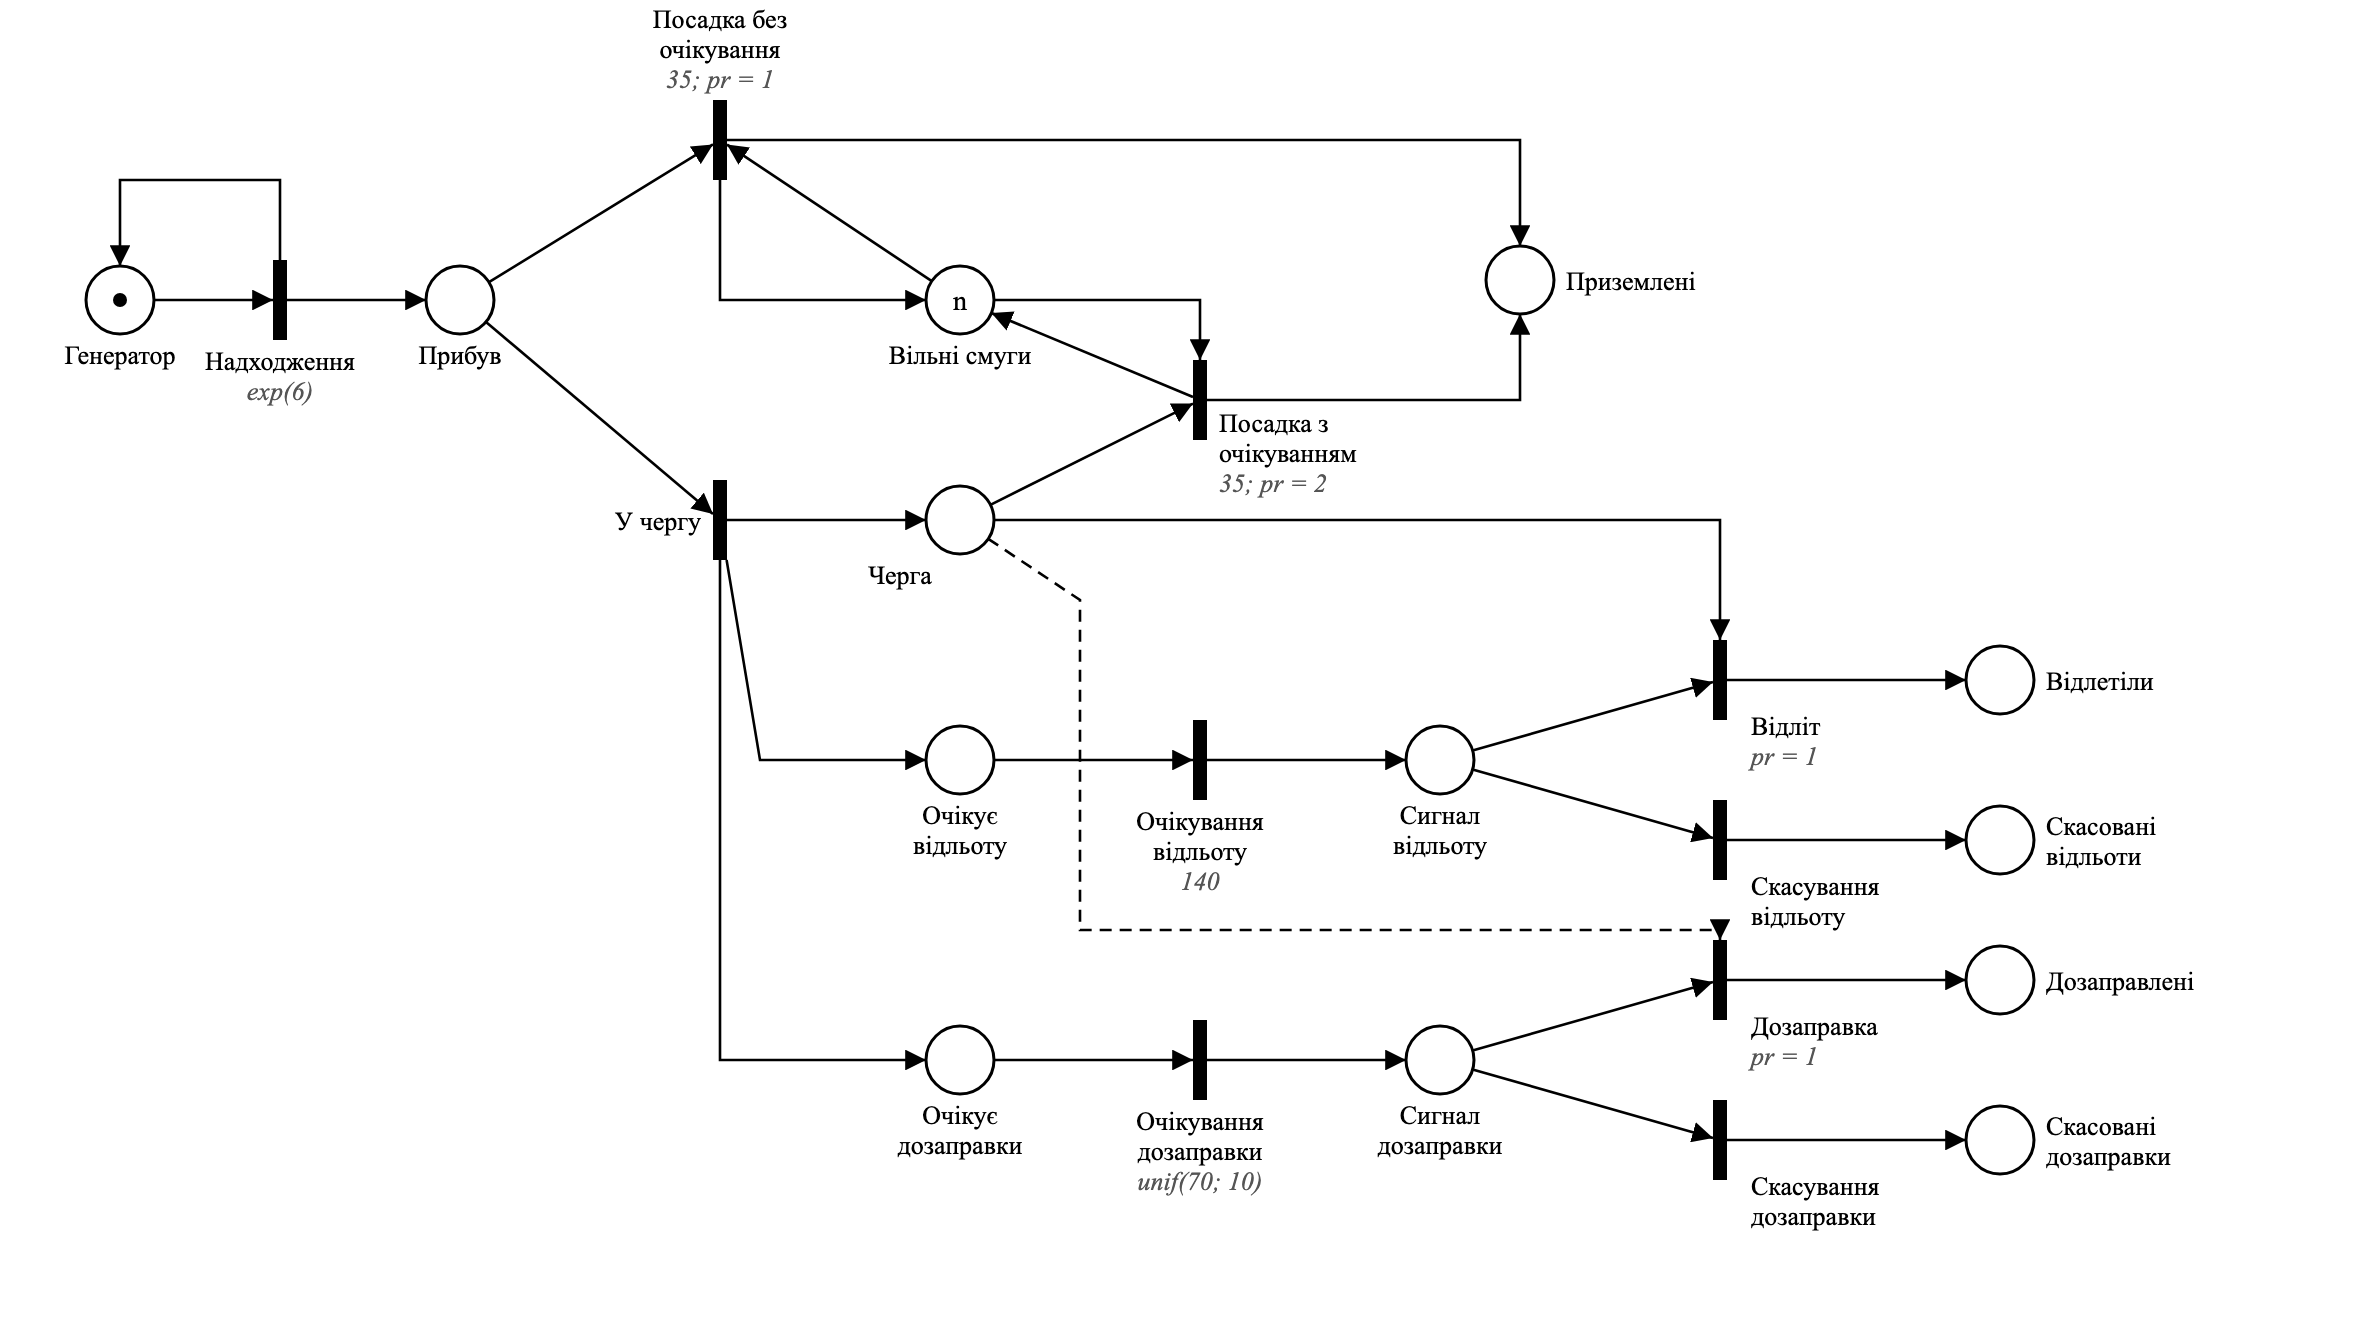
\includegraphics[width=\textwidth]{airport.png}
\caption{Стохастична мережа Петрі моделі аеропорту}
\label{fig:petri}
\end{figure}

Перехід «Надходження» з позицією «Генератор» відтворює пуассонівський потік: інтервали між літаками розподілені експоненційно із середнім 6~хв. Кожен вихід маркера створює новий літак у позиції «Прибув».

Далі з позиції «Прибув» можливі два переходи. «Посадка без очікування» потребує ще й маркера в позиції «Вільні смуги» (спочатку там $n$ маркерів), має пріоритет 1 і тому спрацьовує першим, якщо смуга є. Затримка 35~хв -- час, протягом якого смуга зайнята; після неї маркер повертається у «Вільні смуги», а літак -- у «Приземлені». Якщо вільної смуги немає, спрацьовує перехід «У чергу» з нульовою затримкою. Він кладе той самий літак у три позиції: «Черга», «Очікує відльоту» і «Очікує дозаправки». Так для літака одночасно стартують черга і два таймери.

Перехід «Посадка з очікуванням» бере з «Черги» перший літак і вільну смугу. Його пріоритет 2 вищий, ніж у посадки без очікування, тож звільнена смуга дістається літаку, що вже чекає, а новий літак стає в кінець черги.

Таймер відльоту -- перехід «Очікування відльоту» зі сталою затримкою 140~хв. Після нього літак потрапляє в «Сигнал відльоту». Перехід «Відліт» має дві вхідні дуги match: із «Сигналу відльоту» і з «Черги». Тому він спрацьовує, лише якщо цей самий літак досі в черзі, і забирає його звідти. Якщо літак уже сів, умова «Відльоту» не виконана, і сигнал прибирає перехід «Скасування відльоту» з нижчим пріоритетом 0.

Таймер дозаправки влаштований так само із затримкою $\mathrm{unif}(70; 10)$. Відмінність у тому, що «Дозаправка» перевіряє наявність літака в черзі \emph{інформаційною} дугою: дозаправлений літак лишається в черзі й далі чекає на смугу або на свій відліт.

\begin{kpitable}{|L{4.3cm}|L{2.4cm}|L{8.7cm}|}{Позиції мережі Петрі та їх початкове маркування\label{tab:places}}{\textbf{Позиція} & \textbf{Початкова кількість маркерів} & \textbf{Зміст}}
Генератор & 1 & джерело потоку літаків \\ \hline
Прибув & 0 & літак щойно прибув і потребує посадки \\ \hline
Вільні смуги & $n$ & кількість вільних посадкових смуг \\ \hline
Черга & 0 & літаки, що чекають на посадку, у порядку прибуття \\ \hline
Приземлені & 0 & літаки, що здійснили посадку \\ \hline
Очікує відльоту & 0 & для літака в черзі запущено відлік 140~хв \\ \hline
Сигнал відльоту & 0 & 140~хв минули, треба перевірити, чи літак ще в черзі \\ \hline
Відлетіли & 0 & літаки, що відлетіли в інший аеропорт \\ \hline
Скасовані відльоти & 0 & сигнали відльоту літаків, що встигли сісти \\ \hline
Очікує дозаправки & 0 & для літака в черзі запущено відлік до дозаправки \\ \hline
Сигнал дозаправки & 0 & поріг дозаправки минув, треба перевірити, чи літак ще в черзі \\ \hline
Дозаправлені & 0 & літаки, які дозаправили \\ \hline
Скасовані дозаправки & 0 & сигнали дозаправки літаків, що встигли сісти \\ \hline
\end{kpitable}

\begin{kpitable}{|L{3.9cm}|L{2.7cm}|L{0.8cm}|L{0.8cm}|L{7.2cm}|}{Параметри переходів мережі Петрі\label{tab:transitions}}{\textbf{Перехід} & \textbf{Затримка $d$, хв} & \textbf{$r$} & \textbf{$b$} & \textbf{Вхідні (in) та вихідні (out) позиції}}
Надходження & $\exp(6)$ & 0 & 1 & in: Генератор; out: Генератор, Прибув (carry); створює літак \\ \hline
Посадка без очікування & 35 & 1 & 1 & in: Прибув (match), Вільні смуги; out: Приземлені (carry), Вільні смуги \\ \hline
У чергу & 0 & 0 & 1 & in: Прибув (match); out: Черга, Очікує відльоту, Очікує дозаправки (усі carry) \\ \hline
Посадка з очікуванням & 35 & 2 & 1 & in: Черга (match), Вільні смуги; out: Приземлені (carry), Вільні смуги \\ \hline
Очікування відльоту & 140 & 0 & 1 & in: Очікує відльоту (match); out: Сигнал відльоту (carry) \\ \hline
Відліт & 0 & 1 & 1 & in: Сигнал відльоту (match), Черга (match); out: Відлетіли \\ \hline
Скасування відльоту & 0 & 0 & 1 & in: Сигнал відльоту; out: Скасовані відльоти \\ \hline
Очікування дозаправки & $\mathrm{unif}(70; 10)$ & 0 & 1 & in: Очікує дозаправки (match); out: Сигнал дозаправки (carry) \\ \hline
Дозаправка & 0 & 1 & 1 & in: Сигнал дозаправки (match); інформаційна: Черга (match); out: Дозаправлені \\ \hline
Скасування дозаправки & 0 & 0 & 1 & in: Сигнал дозаправки; out: Скасовані дозаправки \\ \hline
\end{kpitable}

Усі дуги мають кратність 1. Ймовірності запуску в моделі не використовуються: кожен конфлікт розв'язує пріоритет. Конфліктів чотири:
\begin{itemize}
\item «Посадка без очікування» ($r = 1$) і «У чергу» ($r = 0$) за маркер у позиції «Прибув»: літак стає в чергу лише тоді, коли вільних смуг немає;
\item «Посадка з очікуванням» ($r = 2$) і «Посадка без очікування» ($r = 1$) за вільну смугу: першим сідає літак, що вже чекає;
\item «Відліт» ($r = 1$) і «Скасування відльоту» ($r = 0$) за сигнал: сигнал скасовується, лише якщо літака в черзі вже немає;
\item «Дозаправка» ($r = 1$) і «Скасування дозаправки» ($r = 0$) -- так само.
\end{itemize}

\subsection{Формули вихідних характеристик}

Статистика збирається на інтервалі $[T_w; T_w + T_m]$, де $T_w$ -- час розгону, $T_m$ -- тривалість збору статистики. Позначимо $|E_{X}|$ кількість входів маркерів у перехід $X$ на цьому інтервалі. Тоді кількості літаків визначаються так:
\begin{equation}
N_a = |E_{\text{Надходження}}|, \quad N_0 = |E_{\text{Посадка без очікування}}|, \quad N_1 = |E_{\text{Посадка з очікуванням}}|,
\label{eq:counts}
\end{equation}
\[
N_r = |E_{\text{Дозаправка}}|, \quad N_l = |E_{\text{Відліт}}|.
\]

Дохід від посадок і витрати на дозаправку обчислюються за формулами
\begin{equation}
D = c_0 \cdot N_0 + \sum_{i=1}^{N_1} c_{1,i}, \qquad C = \sum_{j=1}^{N_r} z_j,
\label{eq:money}
\end{equation}
де
\begin{where}
c_0 & дохід за посадку без очікування, 2000~грн; \\
c_{1,i} & дохід за $i$-ту посадку з очікуванням, рівномірно на $[1400; 1600]$~грн; \\
z_j & витрати на $j$-ту дозаправку, рівномірно на $[800; 1200]$~грн.
\end{where}

Річний прибуток аеропорту перераховується на рік з 365~діб, тобто 525\,600~хв:
\begin{equation}
P = \frac{D - C}{T_m} \cdot 525\,600.
\label{eq:profit}
\end{equation}

Середній час очікування рахується за всіма літаками, що сіли; для літака без очікування він дорівнює нулю:
\begin{equation}
W = \frac{1}{N_0 + N_1} \sum_{i=1}^{N_1} \left(t^{\text{пос}}_i - t^{\text{пр}}_i\right),
\label{eq:wait}
\end{equation}
де $t^{\text{пр}}_i$ -- момент прибуття $i$-го літака, що сів з очікуванням (момент створення його маркера), $t^{\text{пос}}_i$ -- момент його посадки.

Середня довжина черги і середня кількість зайнятих смуг -- середні в часі значення кусково-сталих величин~\cite{stetsenko2024}:
\begin{equation}
L = \frac{1}{T_m} \sum_{s} M_{\text{Черга}}(t_s) \cdot \Delta t_s,
\label{eq:means}
\end{equation}
\[
B = \frac{1}{T_m} \sum_{s} \left(K_{\text{Посадка без очікування}}(t_s) + K_{\text{Посадка з очікуванням}}(t_s)\right) \cdot \Delta t_s,
\]
де $M_X(t_s)$ -- кількість маркерів у позиції $X$, $K_X(t_s)$ -- кількість зайнятих каналів переходу $X$ на інтервалі $[t_s; t_s + \Delta t_s)$ між сусідніми подіями.

Час окупності обчислюється для кожного прогону моделі з $n = 2 + k$ смугами, і результатом є середнє за прогонами. Основний варіант -- за приростом прибутку порівняно з двома смугами в тому самому прогоні, другий -- за загальним прибутком:
\begin{equation}
T_{\Delta}(n) = \frac{S(n)}{P(n) - P(2)} \cdot 12, \qquad T_{P}(n) = \frac{S(n)}{P(n)} \cdot 12, \qquad S(n) = s \cdot (n - 2),
\label{eq:payback}
\end{equation}
де множник 12 переводить роки в місяці, $s = 3 \cdot 10^6$~грн -- вартість однієї смуги. $T_{P}$ має сенс лише тоді, коли $P(n) > 0$ у кожному прогоні. Оптимальна кількість смуг -- та, за якої середнє $T$ найменше.

\subsection{Висновки до розділу}

Аеропорт описано стохастичною мережею Петрі з 13~позицій і 10~переходів. Щоб кожен літак мав власні таймери дозаправки й відльоту, мережу доповнено маркерами-об'єктами та дугами match і carry; без них таймер одного літака міг би забрати з черги інший. Визначено всі числові параметри: затримки, пріоритети, ймовірності запуску і початкове маркування. Конфлікти переходів розв'язуються пріоритетами. Для вихідних характеристик, зокрема річного прибутку і часу окупності, наведено формули \eqref{eq:counts}--\eqref{eq:payback}.

\section{Алгоритмізація моделі системи та її програмна реалізація}

\subsection{Вибір мови програмування}

Модель реалізовано мовою TypeScript~\cite{typescript} і виконано в середовищі Bun~\cite{bun}. Вибір обумовлено трьома причинами. По-перше, статична типізація TypeScript ловить помилки опису мережі до запуску: наприклад, перехід не може посилатися на позицію іншої мережі, а у вихідних характеристик прогону фіксований набір полів. По-друге, Bun виконує TypeScript без окремої компіляції, має вбудований засіб модульного тестування і достатньо швидкий для серій із сотень прогонів на рік модельного часу. По-третє, та сама програма будує схему мережі (SVG і draw.io) і графіки результатів, тож рисунки у звіті отримано з того самого опису моделі, який імітується.

Бібліотеки імітаційного моделювання не використовувались: алгоритм імітації мережі Петрі, генератори випадкових величин і статистична обробка написані в межах роботи. Готові системи на кшталт Arena~\cite{kelton2024} чи CPN Tools пропонують подібні засоби, але приховують сам алгоритм імітації, а саме його розробка є метою курсової роботи.

\subsection{Структура програми}

Програма складається з модулів, наведених у таблиці~\ref{tab:modules}. Модулі \code{petri.ts}, \code{random.ts} і \code{stats.ts} -- загальні: вони не знають про аеропорт і можуть імітувати будь-яку мережу Петрі. Модуль \code{airport.ts} будує мережу аеропорту і рахує його вихідні характеристики, \code{experiments.ts} -- проводить експерименти. Повний код наведено в додатках~\ref{app:petri}--\ref{app:experiments}.

\begin{kpitable}{|L{4.2cm}|L{11.2cm}|}{Модулі програми\label{tab:modules}}{\textbf{Модуль} & \textbf{Призначення}}
\code{petri.ts} & елементи мережі Петрі (позиція, перехід, дуга, маркер), алгоритм імітації, збір статистики по позиціях і переходах \\ \hline
\code{random.ts} & генератор випадкових чисел і закони розподілу затримок \\ \hline
\code{stats.ts} & вибіркове середнє, стандартне відхилення, довірчий інтервал \\ \hline
\code{airport.ts} & мережа Петрі аеропорту, параметри завдання, обчислення вихідних характеристик прогону \\ \hline
\code{experiments.ts} & перехідний період, кількість прогонів, верифікація, перебір кількості смуг, пробний запуск \\ \hline
\code{schemes.ts}, \code{charts.ts} & побудова схеми мережі й графіків \\ \hline
\code{index.ts} & запуск усіх експериментів і збереження результатів \\ \hline
\end{kpitable}

\subsection{Класи алгоритму імітації}

Діаграму класів наведено на рисунку~\ref{fig:uml}. Класи відповідають елементам формалізму з розділу~2.

\begin{figure}[H]
\centering
\begin{tikzpicture}[
  font=\fontsize{8.5}{10}\selectfont,
  cls/.style={draw, rectangle split, rectangle split parts=3, align=left, text width=4.6cm, inner sep=2.5pt},
  iface/.style={cls, rectangle split parts=2, fill=gray!8},
  assoc/.style={-{Stealth[length=2mm]}},
  comp/.style={{Diamond[length=3mm, width=2mm]}-},
  every node/.append style={node distance=1.0cm},
]
\newcommand\umlname[1]{\makebox[\linewidth][c]{#1}}
\node[iface, anchor=north] (token) at (-5.5, 0) {\umlname{\textit{«interface»} \textbf{Token}}
  \nodepart{second} +id: number\\ +born: number};
\node[cls, anchor=north] (net) at (0, 0) {\umlname{\textbf{Net}}
  \nodepart{second} +places: Place[]\\ +transitions: Transition[]
  \nodepart{third} +place(name, tokens, layout)\\ +transition(name, delay, spec)\\ +reset(): void};
\node[cls, anchor=north] (sim) at (5.5, 0) {\umlname{\textit{«module»} \textbf{petri}}
  \nodepart{second} --
  \nodepart{third} +simulate(net, options): RunResult\\ -enterAll(net, t, rng, onEnter)};
\node[cls, anchor=north] (place) at (-5.5, -3.0) {\umlname{\textbf{Place}}
  \nodepart{second} +name: string\\ +initial: number\\ +tokens: Token[]\\ +count: number
  \nodepart{third} +reset(): void\\ +has(id): boolean\\ +take(id?): Token};
\node[cls, anchor=north] (tr) at (0, -3.0) {\umlname{\textbf{Transition}}
  \nodepart{second} +name: string\\ +delay: Distribution\\ +inputs, outputs, info: Arc[]\\ +priority, probability: number\\ +spawn: boolean\\ +channels: Channel[]\\ +fired: number\\ +busy, nextExit: number
  \nodepart{third} +binding(): Token | undefined | null\\ +enter(t, rng, token): void\\ +exit(t, create): void};
\node[cls, anchor=north] (gauge) at (5.5, -3.0) {\umlname{\textbf{Gauge}}
  \nodepart{second} +max: number\\ +mean: number
  \nodepart{third} +add(dt): void\\ +share(v): number};
\node[iface, anchor=north] (arc) at (-5.5, -7.2) {\umlname{\textit{«interface»} \textbf{Arc}}
  \nodepart{second} +place: Place\\ +weight: number\\ +match, carry: boolean};
\node[iface, anchor=north] (dist) at (5.5, -7.2) {\umlname{\textit{«interface»} \textbf{Distribution}}
  \nodepart{second} +label: string\\ +mean: number\\ +sample(rng): number};
\draw[comp] (net.south) -- (tr.north);
\draw[comp] (net.south west) -- (place.north east);
\draw[assoc] (place.north) -- (token.south);
\draw[assoc] (arc.north) -- (place.south);
\draw[assoc] (tr.west |- arc.north) ++(0,-0.6) -- ($(arc.north east)+(0,-0.6)$);
\draw[assoc] (tr.east |- dist.north) ++(0,-0.6) -- ($(dist.north west)+(0,-0.6)$);
\draw[assoc] (sim.south) -- (gauge.north);
\draw[assoc, dashed] (sim.west) -- (net.east |- sim.west);
\end{tikzpicture}
\caption{Діаграма класів алгоритму імітації мережі Петрі}
\label{fig:uml}
\end{figure}

Клас \code{Place} зберігає маркери позиції у порядку надходження. Безіменний маркер -- об'єкт з номером 0; маркер-літак має номер і момент створення (інтерфейс \code{Token}). Метод \code{take} забирає перший маркер або маркер заданого об'єкта.

Клас \code{Transition} зберігає дуги, параметри $d$, $r$, $b$ і список зайнятих каналів \code{channels}: для кожного каналу -- момент виходу і об'єкт, що в ньому перебуває. Кількість каналів не обмежена, тож перехід багатоканальний. Метод \code{binding} перевіряє умову запуску, \code{enter} здійснює вхід маркерів, \code{exit} -- вихід маркерів з каналів, момент виходу яких настав. Поле \code{fired} рахує виходи.

Інтерфейс \code{Distribution} описує закон розподілу затримки: позначення для схеми, математичне сподівання і функцію генерування значення. Клас \code{Gauge} накопичує середнє в часі значення кусково-сталої величини -- кількості маркерів у позиції чи зайнятих каналів переходу. Функція \code{simulate} реалізує алгоритм імітації, \code{enterAll} -- вхід маркерів у переходи з розв'язанням конфліктів.

\subsection{Алгоритм імітації мережі Петрі}

Алгоритм імітації стохастичної мережі Петрі побудовано за посібником~\cite{stetsenko2024}. Час просувається від події до події: подією є вихід маркерів з переходу. Алгоритм складається з таких кроків:
\begin{enumerate}[label=\arabic*)]
\item повернути мережу в початкове маркування, покласти $t = 0$;
\item здійснити вхід маркерів у переходи (крок 7);
\item знайти момент найближчої події $t_{n} = \min_X \min_c t^{\text{вих}}_{X, c}$ серед моментів виходу всіх зайнятих каналів усіх переходів;
\item якщо $t_{n} > T_{\text{mod}}$, накопичити статистику до $T_{\text{mod}}$ і завершити імітацію;
\item накопичити статистику на інтервалі $[t; t_n)$ (лише після часу розгону) і просунути час: $t = t_n$;
\item для кожного переходу здійснити вихід маркерів з усіх каналів, момент виходу яких дорівнює $t$; на виході перехід-генератор створює новий об'єкт, а дуги carry переносять об'єкт у вихідні позиції;
\item доки є переходи з виконаною умовою запуску: залишити ті з них, що мають найбільший пріоритет; якщо їх кілька, вибрати один випадково з імовірностями, пропорційними $b$; забрати маркери з вхідних позицій і зайняти новий канал з моментом виходу $t + d$, де $d$ -- згенерована затримка;
\item перейти до кроку 3.
\end{enumerate}

Крок 7 повторюється, доки є переходи з виконаною умовою, тому багатоканальний перехід за один момент часу може прийняти стільки маркерів, скільки їх є у вхідних позиціях. Переходи з нульовою затримкою отримують момент виходу $t$ і обробляються на наступній ітерації кроків 3--6 без просування часу. Це дозволяє, наприклад, перевірити сигнал відльоту в той самий момент, коли спрацював таймер. Щоб помилка в описі мережі (цикл переходів з нульовою затримкою) не зависала, кількість входів за один момент обмежена.

Умову запуску з урахуванням маркерів-об'єктів перевіряє метод \code{binding}. Спершу перевіряється кількість маркерів на всіх вхідних та інформаційних дугах, далі для дуг match шукається об'єкт, присутній в усіх відповідних позиціях:
\begin{Verbatim}
binding(): Token | undefined | null {
  const arcs = [...this.inputs, ...this.info];
  if (!arcs.every((a) => a.place.count >= a.weight)) return null;
  const matched = arcs.filter((a) => a.match);
  const [first, ...rest] = matched;
  if (!first) return undefined;
  return first.place.tokens.find((tk) => rest.every((a) => a.place.has(tk.id))) ?? null;
}
\end{Verbatim}
Результат \code{null} означає, що умова не виконана, \code{undefined} -- що перехід працює лише з безіменними маркерами. Оскільки об'єкт шукається в порядку надходження, перехід «Посадка з очікуванням» бере з черги літак, що прибув найраніше.

Розв'язання конфліктів (крок 7) реалізує функція \code{enterAll}:
\begin{Verbatim}
const enabled = net.transitions.flatMap((tr) => {
  const token = tr.binding();
  return token === null ? [] : [{ tr, token }];
});
if (!enabled.length) return;
const top = Math.max(...enabled.map((e) => e.tr.priority));
const rivals = enabled.filter((e) => e.tr.priority === top);
let chosen = rivals[0];
if (rivals.length > 1) {
  let u = rng() * rivals.reduce((s, e) => s + e.tr.probability, 0);
  chosen = rivals.find((e) => (u -= e.tr.probability) < 0) ?? rivals[rivals.length - 1];
}
\end{Verbatim}

Основний цикл (кроки 3--8) у функції \code{simulate}:
\begin{Verbatim}
enterAll(net, t, rng, onEnter);
for (;;) {
  let next = Infinity;
  for (const tr of net.transitions) next = Math.min(next, tr.nextExit);
  if (next > time) {
    advance(time);
    break;
  }
  advance(next);
  for (const tr of net.transitions) tr.exit(t, create);
  enterAll(net, t, rng, onEnter);
  onEvent?.(t);
}
\end{Verbatim}

\subsection{Збір статистики}

Функція \code{advance} просуває час і перед цим додає до кожного об'єкта \code{Gauge} поточне значення величини, помножене на тривалість інтервалу, -- це чисельник формули \eqref{eq:means}. Інтервали до моменту розгону $T_w$ не враховуються, а кількість виходів з переходів відраховується від значення в момент $T_w$.

Дохід і витрати залежать від окремих літаків, тому модуль \code{airport.ts} рахує їх у функції зворотного виклику \code{onEnter}, яку алгоритм викликає при кожному вході маркера в перехід:
\begin{Verbatim}
onEnter: (t, token, now) => {
  if (now < warmup || !token) return;
  if (t === tr.landNow) {
    landedNoWait++;
    income += p.incomeNoWait;
  }
  if (t === tr.landAfterWait) {
    landedAfterWait++;
    income += between(rng, p.incomeWait);
    waitSum += now - token.born;
  }
  if (t === tr.refuel) refuelCosts += between(rng, p.refuelCost);
},
\end{Verbatim}
Час очікування літака -- різниця між моментом посадки і моментом створення його маркера. Річний прибуток обчислюється за формулою \eqref{eq:profit}.

\subsection{Генерування випадкових величин}

Рівномірно розподілені числа на $(0; 1)$ дає генератор mulberry32 з 32-бітним станом. Кожен прогін отримує власне початкове значення (seed), тому будь-який експеримент можна відтворити. Експоненційна затримка генерується методом оберненої функції $x = -d \cdot \ln \xi$, рівномірна на $[a; b]$ -- як $x = a + (b - a) \cdot \xi$, де $\xi$ -- рівномірно розподілене число на $(0; 1)$~\cite{stetsenko2010}. Нуль генератор не повертає, тож логарифм завжди скінченний.

\subsection{Тестування алгоритму імітації}

Алгоритм перевірено модульними тестами (засіб \code{bun test}), усі 10 тестів проходять:
\begin{itemize}
\item мережа Петрі, що відтворює СМО M/M/1 із завантаженням 0,5, дає завантаження пристрою 0,5 і середню довжину черги 0,5, як за теоретичними формулами;
\item перехід з вищим пріоритетом спрацьовує завжди, навіть з ймовірністю запуску 0,01;
\item багатоканальний перехід приймає всі три маркери вхідної позиції одночасно;
\item генератор створює об'єкти з послідовними номерами і моментами створення;
\item дуги match беруть маркери одного об'єкта, навіть якщо він не перший у черзі позиції;
\item інформаційна дуга match перевіряє наявність саме цього об'єкта і не забирає його;
\item у моделі аеропорту кожен літак, що прибув, або сів, або відлетів, або ще чекає;
\item літаки дозаправляються лише після 60--80~хв очікування, а відлітають рівно через 140~хв;
\item за 12~смуг жоден літак не дозаправляється і не відлітає;
\item за 30~смуг усі посадки без очікування, і дохід дорівнює $2000 \cdot N_0$.
\end{itemize}

\subsection{Верифікація моделі}

Верифікація перевіряє, що алгоритм імітації відтворює функціонування системи так, як воно описане. Модель запускалась з вісьмома наборами вхідних даних; у кожному змінювався один параметр. Час моделювання -- 30~діб (43\,200~хв), з них перша доба -- розгін, тобто статистика зібрана за $T_m = 41\,760$~хв. Параметри, не вказані в таблиці, мають значення з таблиці~\ref{tab:inputs}. Результати наведено в таблиці~\ref{tab:verify}. Очікувану кількість надходжень обчислено як $T_m / 6$, очікувану кількість зайнятих смуг -- за формулою Літтла $B = (N_0 + N_1) \cdot t_s / T_m$.

\begingroup
\fontsize{12}{14}\selectfont
\begin{kpitable}{|L{2.6cm}|L{1.7cm}|L{1.0cm}|L{1.1cm}|L{1.1cm}|L{1.1cm}|L{1.0cm}|L{0.9cm}|L{1.8cm}|L{1.4cm}|}{Результати верифікації моделі ($T_m = 41\,760$~хв)\label{tab:verify}}{\textbf{Вхідні дані} & \textbf{$N_a$ (очік.)} & \textbf{$N_0$} & \textbf{$N_1$} & \textbf{$N_r$} & \textbf{$N_l$} & \textbf{$W$, хв} & \textbf{$L$} & \textbf{$B$ (Літтл)} & \textbf{$P$, млн грн/рік}}
базовий & 7148 (6960) & 0 & 2386 & 7137 & 4753 & 133,3 & 23,5 & 2,000 (2,000) & \textminus{}44,62 \\ \hline
$n = 7$ & 6893 (6960) & 3358 & 3543 & 13 & 0 & 7,5 & 1,2 & 5,786 (5,784) & 151,21 \\ \hline
$n = 30$ & 7151 (6960) & 7151 & 0 & 0 & 0 & 0,0 & 0,0 & 5,991 (5,993) & 180,01 \\ \hline
інтервал 12 хв & 3384 (3480) & 5 & 2379 & 3230 & 1001 & 115,5 & 9,9 & 1,999 (1,998) & 4,29 \\ \hline
посадка 20 хв & 7082 (6960) & 0 & 4176 & 7081 & 2911 & 131,3 & 22,9 & 2,000 (2,000) & \textminus{}10,36 \\ \hline
відліт після 90 хв & 6990 (6960) & 0 & 2386 & 6838 & 4602 & 83,7 & 14,7 & 2,000 (2,000) & \textminus{}40,87 \\ \hline
дозаправка після 150 $\pm$ 10 хв & 7080 (6960) & 0 & 2386 & 0 & 4695 & 133,5 & 23,4 & 2,000 (2,000) & 45,08 \\ \hline
дозаправка після 10 $\pm$ 0 хв & 6929 (6960) & 0 & 2386 & 6928 & 4539 & 133,3 & 22,8 & 2,000 (2,000) & \textminus{}41,85 \\ \hline

\end{kpitable}
\endgroup

Результати відповідають очікуваним:
\begin{itemize}
\item кількість літаків, що прибули, відрізняється від очікуваної не більше ніж на 3~\%; для пуассонівського потоку з середнім 6960 це в межах трьох стандартних відхилень ($\sqrt{6960} \approx 83$);
\item середня кількість зайнятих смуг, виміряна в часі, збігається з розрахованою за формулою Літтла до третього знака, тобто посадки і зайнятість смуг узгоджені;
\item за двох смуг обидві смуги зайняті весь час ($B = 2$), і кількість посадок дорівнює найбільшій можливій пропускній здатності $2 \cdot T_m / 35 = 2386$; за посадки 20~хв вона зростає до $2 \cdot T_m / 20 = 4176$;
\item за 30~смуг черги немає зовсім, і всі посадки без очікування;
\item якщо літаки відлітають через 90~хв, середнє очікування не перевищує 90~хв, і відлітає менше літаків;
\item якщо поріг дозаправки більший за час відльоту, дозаправок немає, і прибуток стає додатним; якщо поріг 10~хв, дозаправляють майже кожен літак, що став у чергу;
\item кожен літак, що прибув, або сів, або відлетів: $N_0 + N_1 + N_l$ відрізняється від $N_a$ лише на кількість літаків, що були в черзі на початку й наприкінці інтервалу збору статистики.
\end{itemize}

\subsection{Висновки до розділу}

Алгоритм імітації стохастичної мережі Петрі з маркерами-об'єктами реалізовано мовою TypeScript без бібліотек імітаційного моделювання. Час просувається від події до події, конфлікти розв'язуються за пріоритетом і ймовірністю запуску, переходи багатоканальні. Статистика по позиціях і переходах збирається як середнє в часі, дохід і витрати -- за окремими літаками. Модульні тести підтверджують коректність алгоритму на мережах з відомими теоретичними результатами, а верифікація на восьми наборах вхідних даних -- коректність моделі аеропорту.

\section{Експериментальне дослідження моделі}
\label{sec:experiment}

\subsection{Мета експериментального дослідження}

Мета дослідження задана умовою: знайти кількість посадкових смуг $n$, за якої час окупності додаткових смуг $T$ мінімальний. Отже, модель використовується для оптимізації з одним фактором -- кількістю смуг $n = 2 + k$, де $k = 0, \ldots, 10$ -- і відгуком $T$, обчисленим за формулою \eqref{eq:payback}. Фактор дискретний і має лише 11~значень, тому оптимум шукається повним перебором усіх значень~\cite{stetsenko2024}.

Час окупності обчислюється з річного прибутку $P$, тому умови одного експерименту (тривалість прогону, розгін, кількість повторних прогонів) визначено саме для $P$. Прибуток є відгуком, що стабілізується з часом: це середня швидкість накопичення грошей, на відміну, наприклад, від кількості посадок, що зростає разом із часом моделювання.

Корисно оцінити завантаження смуг: літаки займають у середньому $\lambda \cdot t_s = 35/6 \approx 5{,}83$~смуги. Отже, за $n \le 5$ смуги перевантажені, черга обмежена лише тим, що літаки відлітають після 140~хв, а за $n \ge 6$ смуг вистачає для всього потоку, і черга стає короткою. Цим пояснюється різкий перелом у результатах між $n = 5$ і $n = 7$.

\subsection{Перехідний період і тривалість прогону}

На початку прогону аеропорт порожній: черги немає, і перші літаки сідають без очікування. Такий стан нетиповий для двох смуг, де в сталому режимі черга тримається близько 23~літаків. Щоб визначити тривалість перехідного періоду й тривалість прогону, проведено 4~пробні прогони на 120~діб для $n = 2$ і $n = 7$ і на кожну добу $t$ обчислено оцінку річного прибутку за інтервалом $[0; t]$. Тривалість прогону $T_{\text{mod}}$ визначається умовою~\cite{stetsenko2024}
\begin{equation}
T_{\text{mod}}: \ \forall i, j \quad |y_i(T_{\text{mod}}) - y_j(T_{\text{mod}})| < \varepsilon,
\label{eq:transient}
\end{equation}
де $y_i(t)$ -- оцінка відгуку в $i$-му прогоні за інтервалом $[0; t]$, $\varepsilon$ -- задана точність. Тут $\varepsilon$ узято рівним 2~\% середнього значення оцінки.

Результати наведено на рисунках~\ref{fig:transient-2} і~\ref{fig:transient-7}. За $n = 2$ оцінки чотирьох прогонів відрізняються менше ніж на 2~\% від 91-ї доби, за $n = 7$ -- від 28-ї доби. Тривалість прогону прийнято з запасом рівною одному року модельного часу (525\,600~хв). Рік ще й зручний тим, що прибуток за прогін і є річним прибутком $p$ з формули окупності.

\begin{figure}[H]
\centering
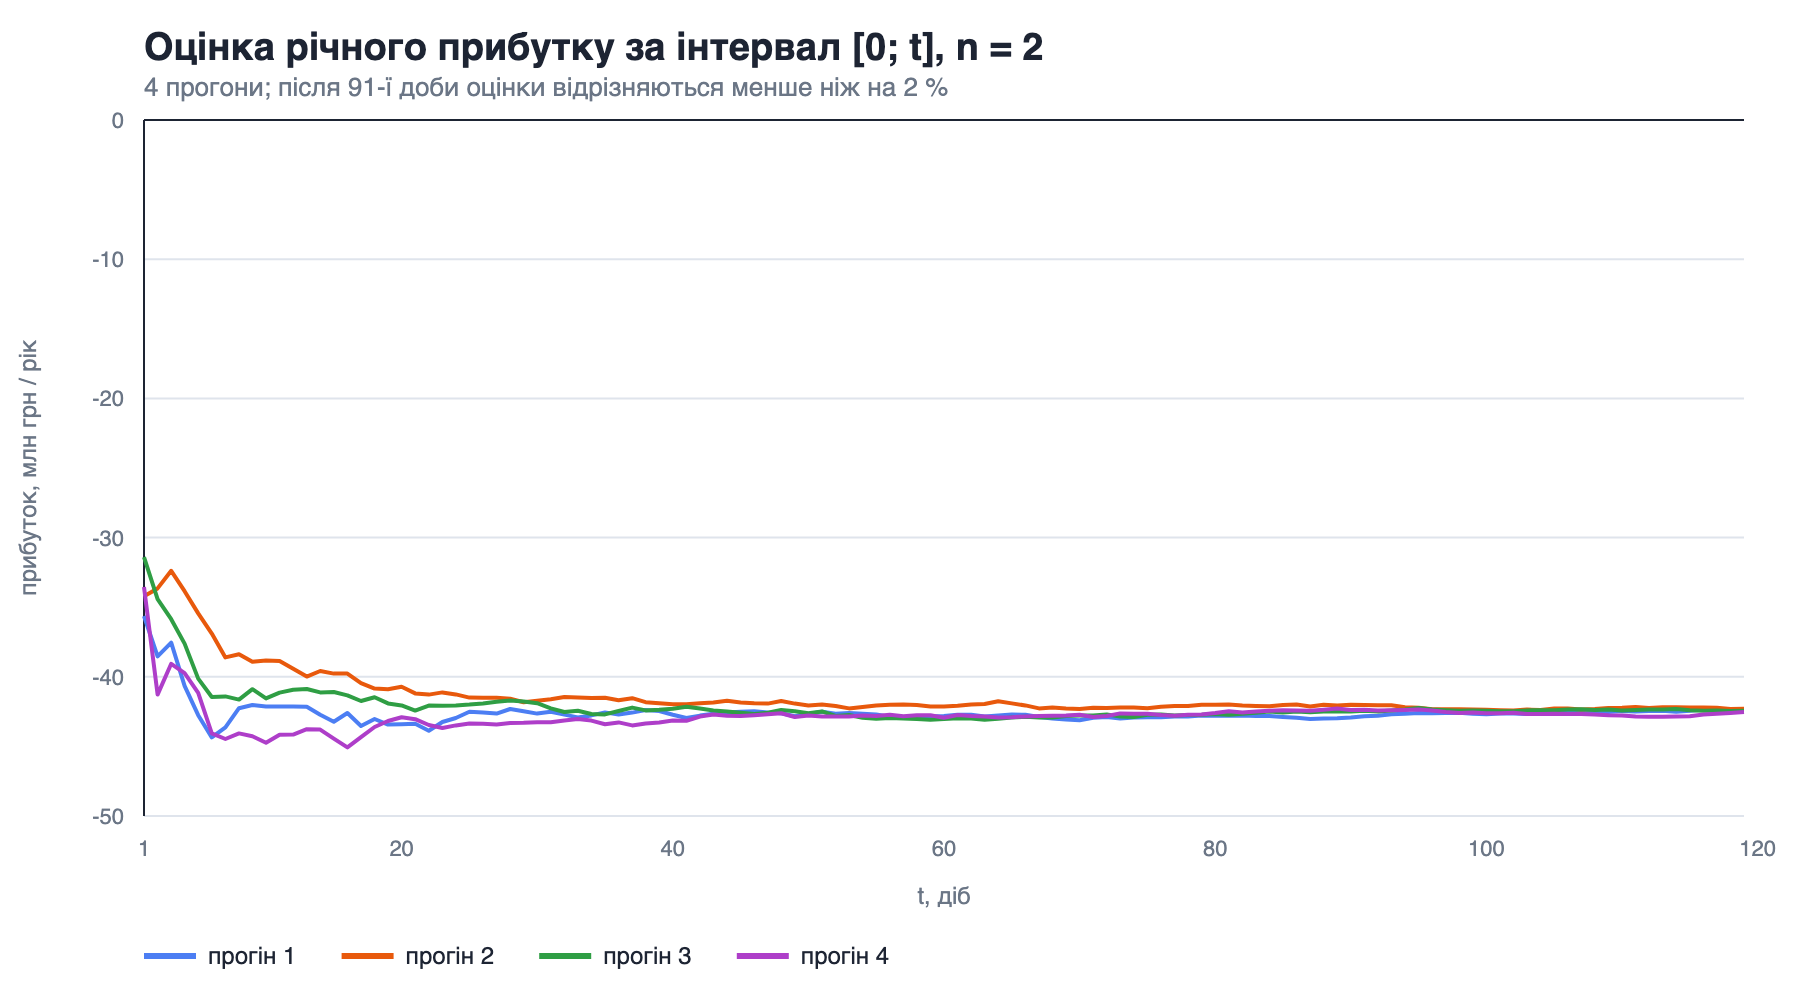
\includegraphics[width=0.92\textwidth]{transient-2.png}
\caption{Оцінка річного прибутку за інтервал $[0; t]$ у чотирьох прогонах, $n = 2$}
\label{fig:transient-2}
\end{figure}

\begin{figure}[H]
\centering
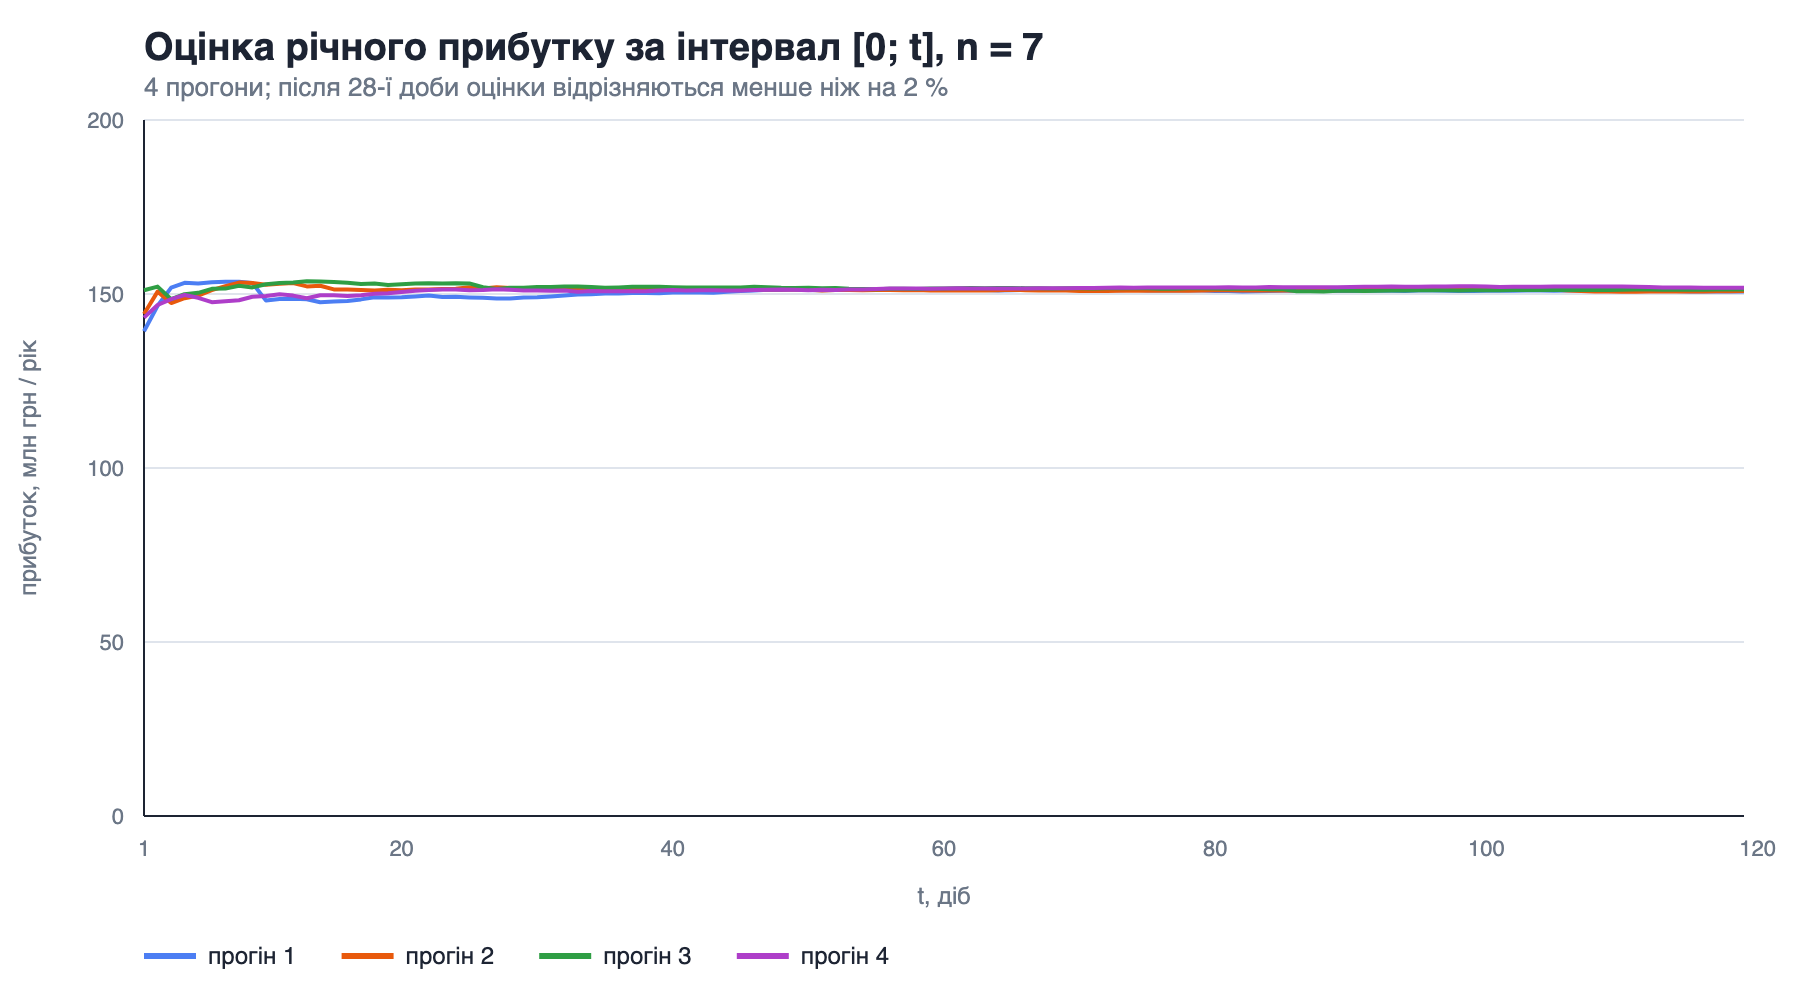
\includegraphics[width=0.92\textwidth]{transient-7.png}
\caption{Оцінка річного прибутку за інтервал $[0; t]$ у чотирьох прогонах, $n = 7$}
\label{fig:transient-7}
\end{figure}

Сам перехідний період значно коротший. На рисунку~\ref{fig:transient-hourly} показано прибуток за кожну годину перших двох діб, усереднений за чотирма прогонами. Нетиповими є лише перші 2--3~години: черга ще не накопичилась, дозаправок немає, і прибуток за годину завищений. Щоб ці години не впливали на результат, статистика збирається після розгону тривалістю одна доба (1440~хв). Отже, кожен прогін триває $T_w + T_m = 1440 + 525\,600 = 527\,040$~хв.

\begin{figure}[H]
\centering
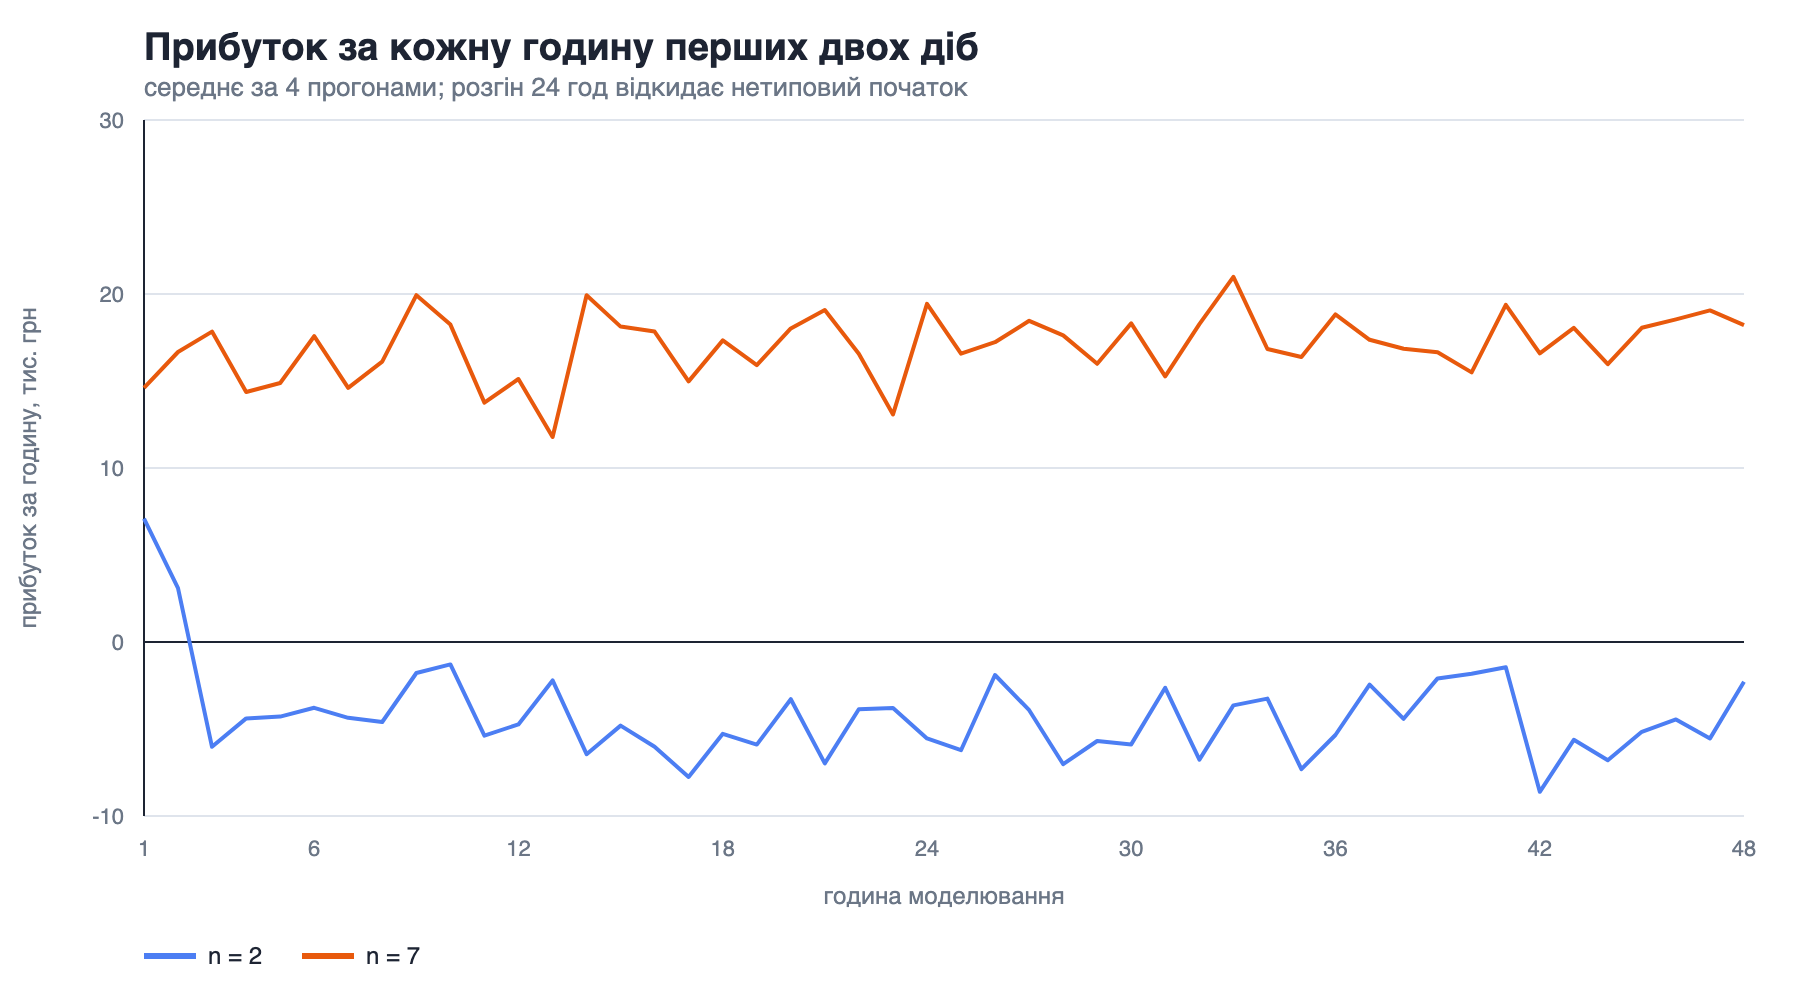
\includegraphics[width=0.92\textwidth]{transient-hourly.png}
\caption{Прибуток аеропорту за кожну годину перших двох діб}
\label{fig:transient-hourly}
\end{figure}

\subsection{Кількість повторних прогонів}

Кількість прогонів, що забезпечує точність $\varepsilon$ з довірчою ймовірністю $\beta = 0{,}95$, визначається наслідком нерівності Чебишева~\cite{stetsenko2024}:
\begin{equation}
p = \frac{\sigma^2}{\varepsilon^2 (1 - \beta)} = 20 \cdot \frac{\sigma^2}{\varepsilon^2},
\label{eq:runs}
\end{equation}
де $\sigma$ -- стандартне відхилення річного прибутку між прогонами, оцінене за 10~пробними прогонами для кожної кількості смуг.

Точність задано в абсолютних одиницях: $\varepsilon = 1$~млн~грн/рік. Відносна точність тут непридатна, бо за чотирьох смуг прибуток близький до нуля (2,6~млн~грн/рік), і 2~\% від нього вимагали б тисяч прогонів. Похибка в 1~млн~грн/рік відповідає менш ніж 1~\% прибутку за $n \ge 6$ і в рази менша за різницю прибутків між сусідніми значеннями $n$ (таблиця~\ref{tab:payback}), тож вона не може змінити вибір оптимуму.

\begin{kpitable}{|L{3.0cm}|L{4.4cm}|L{4.4cm}|L{3.6cm}|}{Кількість прогонів для точності 1~млн~грн/рік\label{tab:runs}}{\textbf{Кількість смуг $n$} & \textbf{Середній прибуток, млн грн/рік} & \textbf{$\sigma$, млн грн/рік} & \textbf{Потрібно прогонів $p$}}
2 & \textminus{}42,476 & 0,259 & 2 \\ \hline
3 & \textminus{}19,941 & 0,216 & 1 \\ \hline
4 & 2,615 & 0,244 & 2 \\ \hline
5 & 28,703 & 0,527 & 6 \\ \hline
6 & 108,146 & 1,587 & 51 \\ \hline
7 & 151,229 & 0,235 & 2 \\ \hline
8 & 162,273 & 0,243 & 2 \\ \hline
9 & 168,386 & 0,293 & 2 \\ \hline
10 & 171,700 & 0,508 & 6 \\ \hline
11 & 173,567 & 0,390 & 4 \\ \hline
12 & 174,477 & 0,606 & 8 \\ \hline

\end{kpitable}

Результати наведено в таблиці~\ref{tab:runs}. Найбільший розкид має $n = 6$: за цієї кількості смуг їх завантаження близьке до одиниці (5,83 з 6), і черга то накопичується, то розсмоктується, тож прибуток окремого року сильно залежить від випадку. Для неї потрібен 51~прогін; цю кількість прийнято для всіх значень $n$, щоб точність була не гіршою за задану для кожного з них.

\subsection{Метод і послідовність експериментів}

Для кожного $k = 0, \ldots, 10$ проведено 51~прогін моделі з $n = 2 + k$ смугами, тривалістю 527\,040~хв кожен, зі збором статистики після першої доби. Загалом це 561~прогін, або 561~рік модельного часу.

Прогони з однаковим номером $i$ для всіх $n$ використовують однакове початкове значення генератора (метод спільних випадкових чисел~\cite{law2015}). Аеропорти з різною кількістю смуг тоді отримують однаковий потік літаків, і різниця прибутків $P(n) - P(2)$ залежить від кількості смуг, а не від того, що одному з варіантів випало більше літаків. Тому час окупності $T_{\Delta}$ обчислюється в кожному прогоні окремо, з прибутків тієї самої пари прогонів, а результатом є середнє за 51~значенням і половина ширини 95~\% довірчого інтервалу за розподілом Стьюдента.

Експерименти проводить функція \code{payback} модуля \code{experiments.ts}:
\begin{Verbatim}
const samples = Array.from({ length: MAX_EXTRA_RUNWAYS + 1 }, (_, extra) =>
  Array.from({ length: runs }, (_, i) =>
    run({ ...params, runways: params.runways + extra }, seed + i)),
);
const base = samples[0] ?? [];
return samples.map((rs, extra) => {
  const cost = extra * params.runwayCost;
  const gains = rs.map((r, i) => r.yearProfit - (base[i]?.yearProfit ?? 0));
  ...
  paybackGain: extra ? estimate(gains.map((g) => cost / g)) : undefined,
\end{Verbatim}
Повний код експериментів наведено в додатку~\ref{app:experiments}. Усі експерименти разом із побудовою графіків запускає команда \code{bun run start}.

\subsection{Результати експериментів}

Середні значення вихідних характеристик за 51~прогоном наведено в таблиці~\ref{tab:payback}. Кількості літаків наведено за рік модельного часу.

\begingroup
\fontsize{12}{14}\selectfont
\begin{kpitable}{|L{0.6cm}|L{1.7cm}|L{1.6cm}|L{1.3cm}|L{1.3cm}|L{1.3cm}|L{1.0cm}|L{1.0cm}|L{2.7cm}|L{1.4cm}|}{Результати перебору кількості смуг (51~прогін по 365~діб)\label{tab:payback}}{\textbf{$n$} & \textbf{$P$, млн грн/рік} & \textbf{$\Delta P$, млн грн/рік} & \textbf{$N_a$} & \textbf{$N_l$} & \textbf{$N_r$} & \textbf{$W$, хв} & \textbf{$B$} & \textbf{$T_{\Delta}$, міс.} & \textbf{$T_P$, міс.}}
2 & \textminus{}42,50 & 0,00 & 87547 & 57511 & 87544 & 132,1 & 2,000 & -- & -- \\ \hline
3 & \textminus{}20,01 & 22,49 & 87615 & 42564 & 87597 & 130,0 & 3,000 & 1,601 $\pm$ 0,007 & -- \\ \hline
4 & 2,63 & 45,12 & 87641 & 27574 & 87479 & 126,9 & 4,000 & 1,596 $\pm$ 0,004 & 27,809 \\ \hline
5 & 28,59 & 71,09 & 87589 & 12519 & 84041 & 116,5 & 4,999 & 1,519 $\pm$ 0,004 & 3,779 \\ \hline
6 & 107,68 & 150,17 & 87526 & 786 & 27218 & 49,4 & 5,776 & 0,959 $\pm$ 0,004 & 1,338 \\ \hline
7 & 151,24 & 193,74 & 87607 & 0 & 479 & 8,8 & 5,834 & 0,929 $\pm$ 0,001 & 1,190 \\ \hline
8 & 162,18 & 204,68 & 87647 & 0 & 6 & 2,9 & 5,836 & 1,055 $\pm$ 0,001 & 1,332 \\ \hline
9 & 168,27 & 210,76 & 87572 & 0 & 0 & 1,1 & 5,831 & 1,196 $\pm$ 0,001 & 1,498 \\ \hline
10 & 171,70 & 214,20 & 87599 & 0 & 0 & 0,4 & 5,833 & 1,345 $\pm$ 0,001 & 1,677 \\ \hline
11 & 173,50 & 216,00 & 87576 & 0 & 0 & 0,2 & 5,832 & 1,500 $\pm$ 0,001 & 1,867 \\ \hline
12 & 174,46 & 216,96 & 87601 & 0 & 0 & 0,1 & 5,833 & 1,659 $\pm$ 0,001 & 2,064 \\ \hline

\end{kpitable}
\endgroup

Залежність прибутку від кількості смуг показано на рисунку~\ref{fig:profit}. За двох смуг аеропорт збитковий: $-42{,}5$~млн~грн/рік. Причина видно з таблиці~\ref{tab:payback}: майже кожен літак, що прибув, стає в чергу і дозаправляється (87\,544 дозаправки на 87\,547 літаків), а сідають лише ті близько 30\,000 літаків на рік, яких можуть прийняти дві смуги ($2 \cdot 525\,600 / 35 \approx 30\,034$); решта 57\,511 відлітають. Витрати на дозаправку всіх літаків перевищують дохід від тих, що сіли. З кожною новою смугою прибуток зростає, найшвидше -- між $n = 5$ і $n = 7$, коли смуг стає достатньо для всього потоку. Після $n = 7$ відльотів уже немає, і кожна наступна смуга лише трохи скорочує очікування, тому приріст прибутку швидко зменшується.

\begin{figure}[H]
\centering
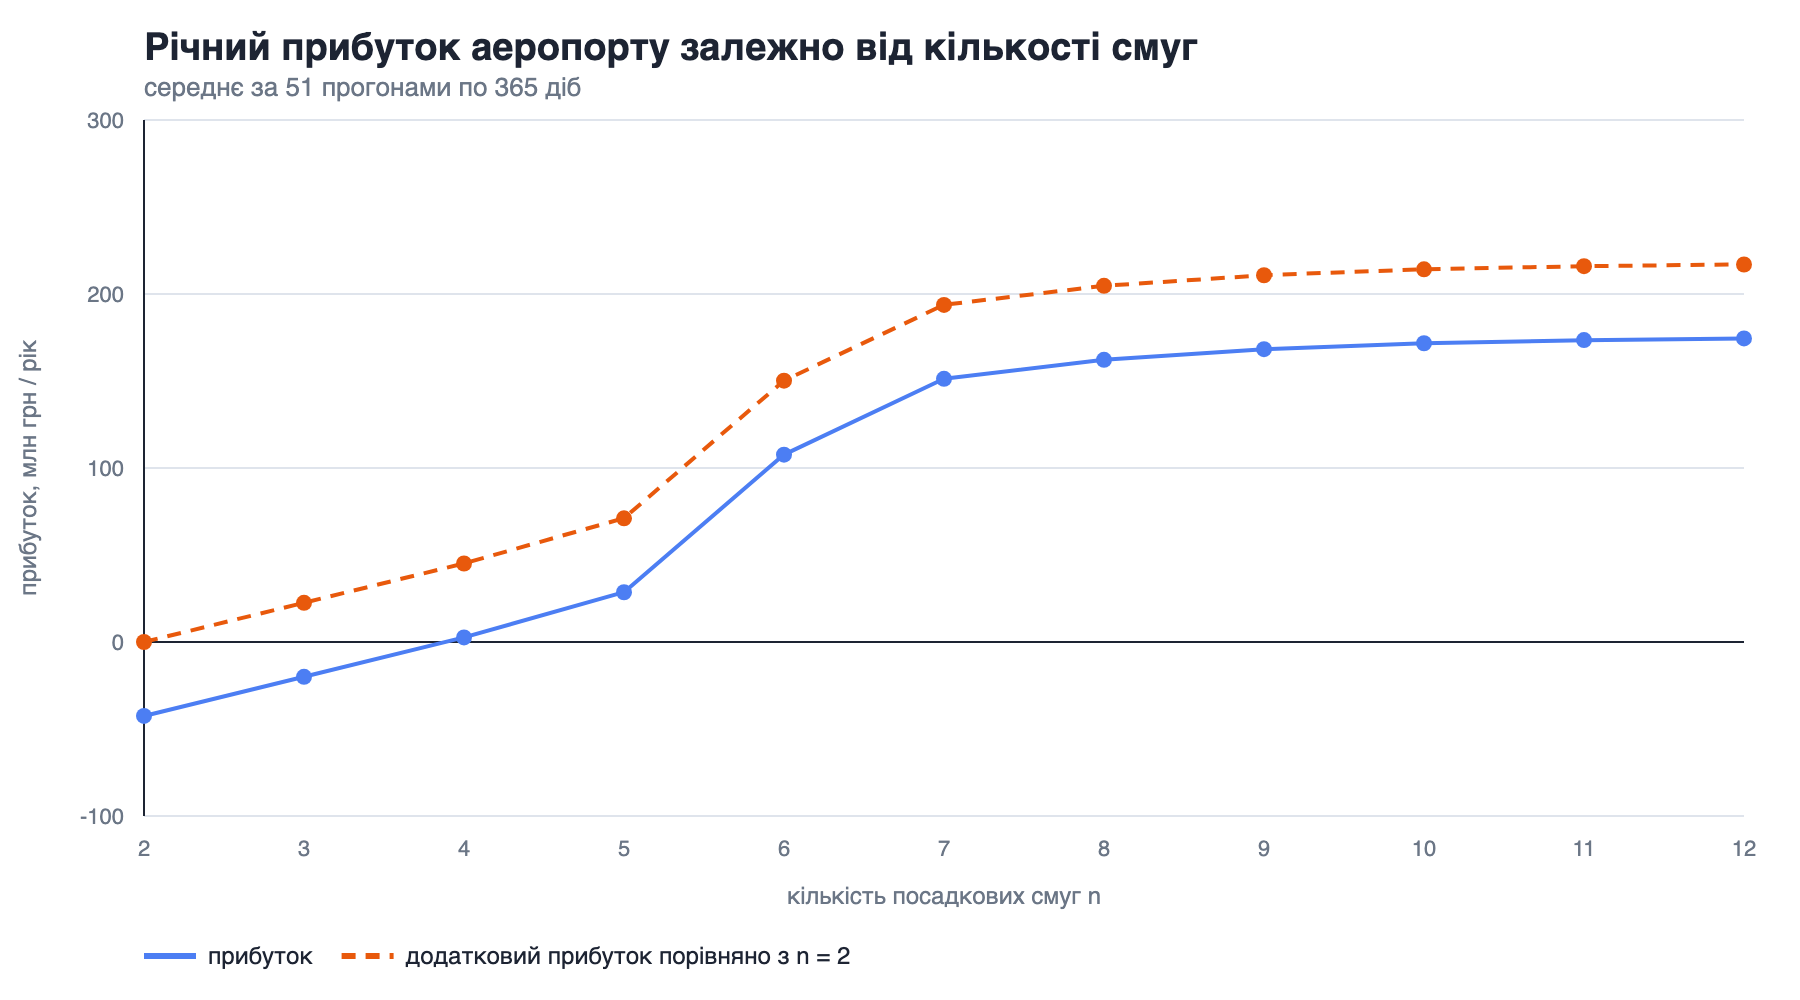
\includegraphics[width=0.92\textwidth]{profit.png}
\caption{Річний прибуток аеропорту залежно від кількості смуг}
\label{fig:profit}
\end{figure}

Як змінюється доля літаків, показано на рисунку~\ref{fig:outcomes}. Частка літаків, що відлітають, падає з 66~\% за двох смуг до нуля за семи; частка дозаправлених -- зі 100~\% до 0,5~\%.

\begin{figure}[H]
\centering
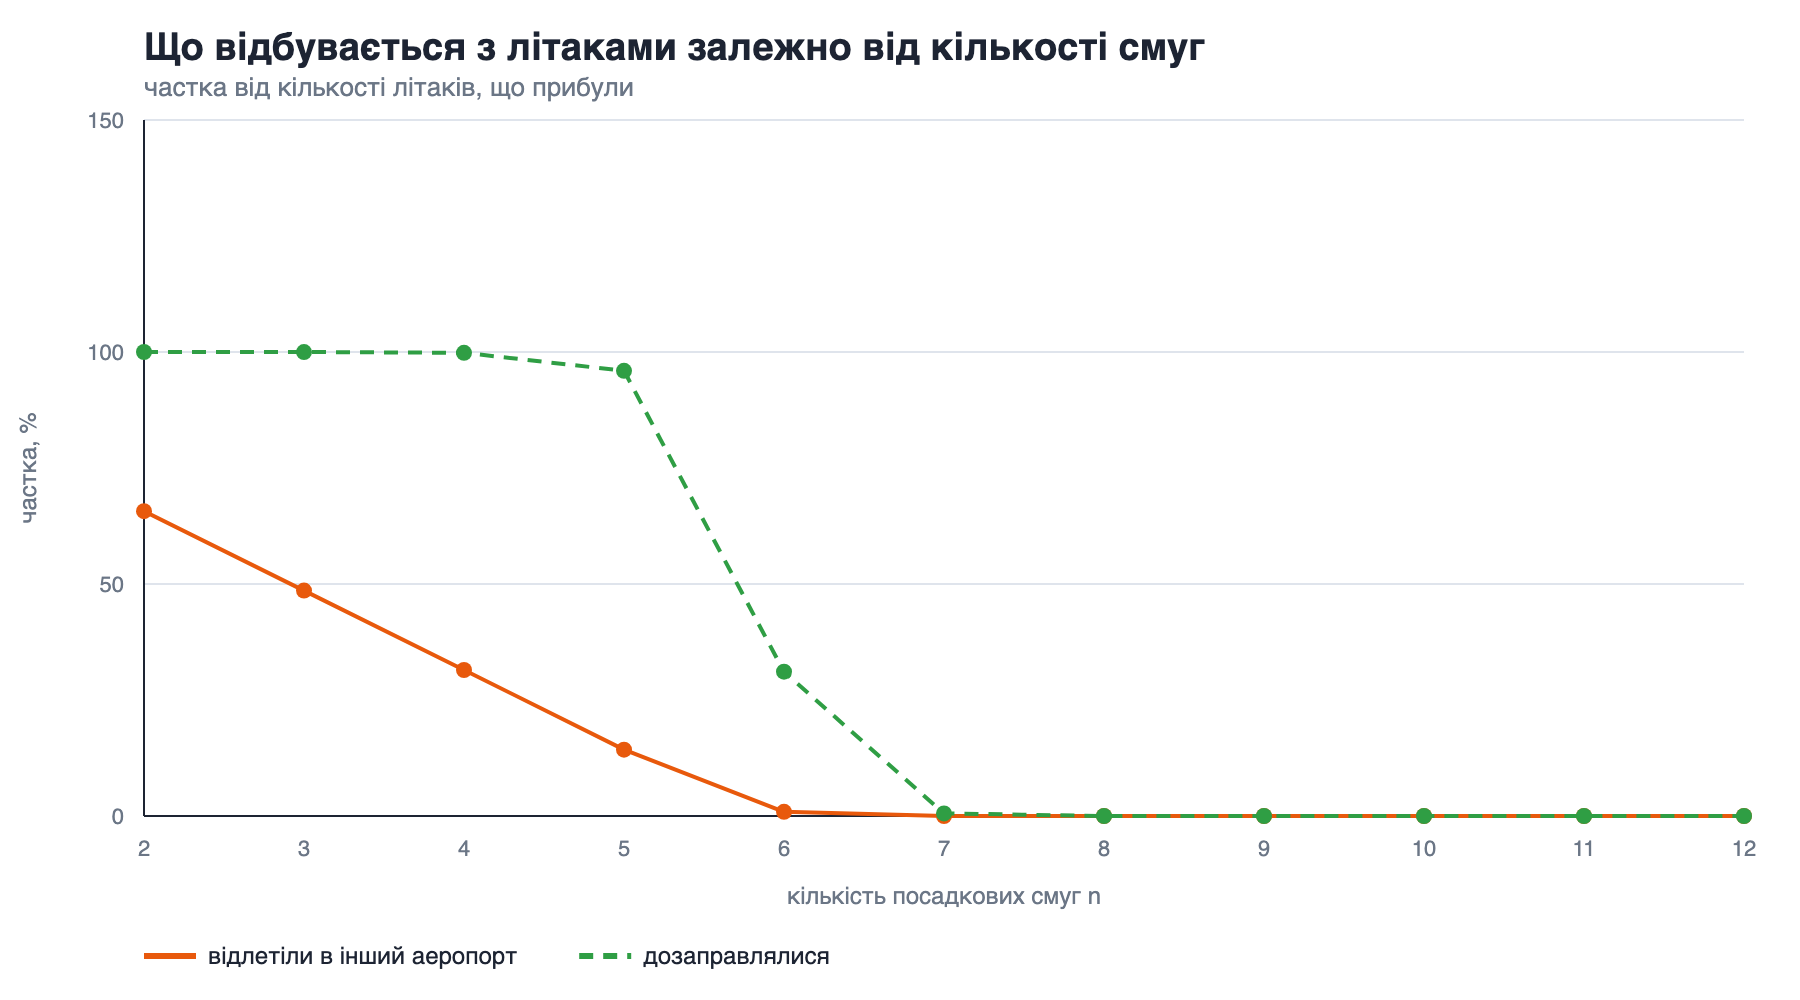
\includegraphics[width=0.92\textwidth]{outcomes.png}
\caption{Частки літаків, що відлетіли й дозаправлялися, залежно від кількості смуг}
\label{fig:outcomes}
\end{figure}

Час окупності показано на рисунку~\ref{fig:payback}. Витрати на смуги зростають лінійно, а приріст прибутку -- спершу швидко, потім дедалі повільніше, тому $T$ має мінімум. За обома інтерпретаціями прибутку $p$ мінімум досягається за $n = 7$: $T_{\Delta} = 0{,}929$~міс. і $T_P = 1{,}190$~міс. Найближчі сусіди, $n = 6$ і $n = 8$, дають $T_{\Delta} = 0{,}959$ і 1,055~міс. Половина ширини довірчого інтервалу для $T_{\Delta}$ не перевищує 0,007~міс. (таблиця~\ref{tab:payback}), тобто довірчі інтервали сусідніх варіантів не перетинаються, і оптимум визначено надійно.

\begin{figure}[H]
\centering
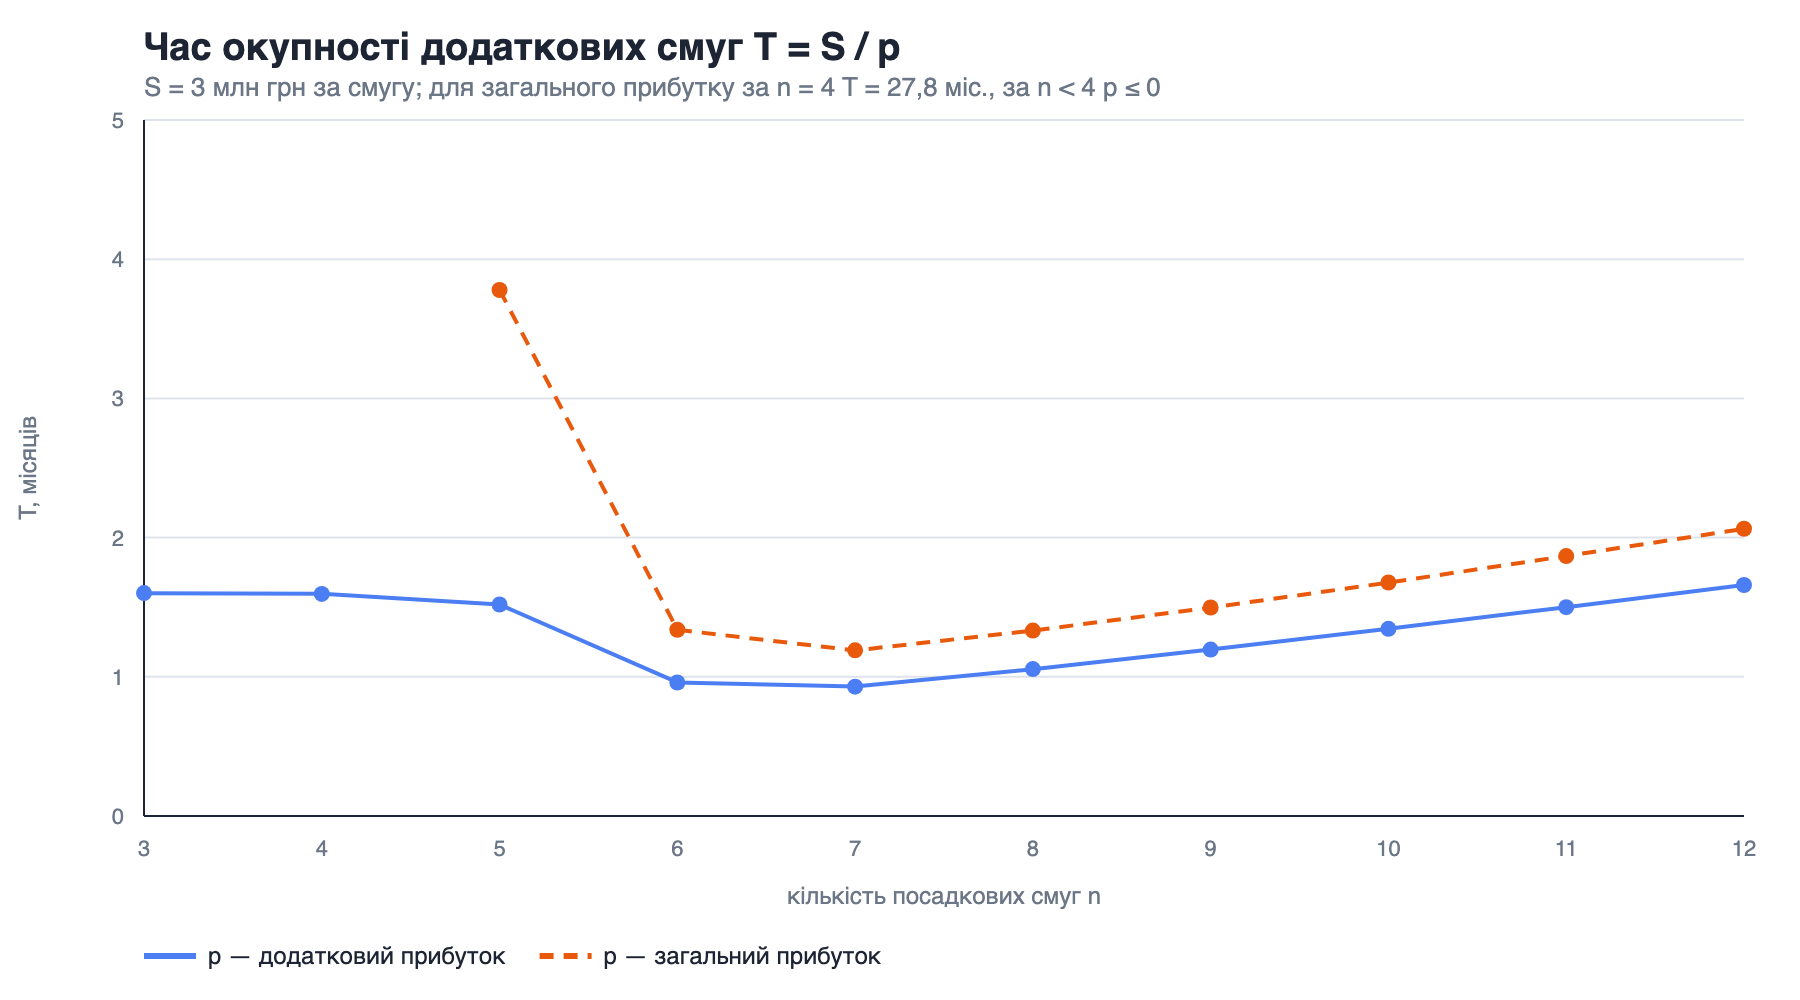
\includegraphics[width=0.92\textwidth]{payback.png}
\caption{Час окупності додаткових смуг залежно від кількості смуг}
\label{fig:payback}
\end{figure}

\subsection{Висновки до розділу}

Визначено умови одного експерименту: прогін тривалістю рік модельного часу після розгону на одну добу, що відкидає нетиповий початок. Для точності 1~млн~грн/рік з довірчою ймовірністю 0,95 потрібен 51~прогін. Повним перебором 11~варіантів з методом спільних випадкових чисел встановлено, що час окупності мінімальний за семи смуг, тобто за п'яти додаткових: 0,929~міс. за приростом прибутку і 1,190~міс. за загальним прибутком.

\section{Інтерпретація результатів моделювання}

\subsection{Інтерпретація результатів}

Двох смуг аеропорту недостатньо. Щоб посадити 10~літаків за годину, кожен з яких займає смугу на 35~хвилин, потрібно в середньому 5,83~смуги, а їх лише дві. Тому черга росте, доки її не обмежує відліт літаків через 140~хвилин. У такому режимі майже кожен літак чекає довше за поріг дозаправки, тож аеропорт платить за дозаправку кожного, а дохід отримує лише за третину з них. Витрати на дозаправку (близько 1000~грн) переважують дохід від посадки з очікуванням (близько 1500~грн), помножений на частку тих, хто сів. Звідси збиток 42,5~млн~грн на рік.

Третя, четверта і п'ята смуги збільшують прибуток на 22--26~млн~грн кожна: кожна приймає ще близько 15\,000~літаків на рік, але смуги все ще перевантажені, і майже всі літаки дозаправляються. Перелом настає між п'ятою і сьомою смугами, коли пропускна здатність смуг перевищує потік літаків: черга зникає, дозаправки й відльоти припиняються, і прибуток стрибає з 28,6 до 151,2~млн~грн на рік. Після семи смуг прибуток зростає ледь помітно, бо майже всі літаки й так сідають і зростає лише частка посадок без очікування (2000~грн замість 1500).

Тому час окупності має чіткий мінімум на семи смугах. Будівництво п'яти додаткових смуг коштує 15~млн~грн і дає приріст прибутку 193,7~млн~грн на рік, тобто окупається за 0,93~місяця, або близько 28~діб. Шоста смуга окупилась би за 0,96~місяця, восьма -- за 1,06~місяця. Ці різниці невеликі в абсолютних числах, але довірчі інтервали не перетинаються, тож сім смуг -- справді найкращий варіант за умовами завдання.

\subsection{Пропозиції щодо поліпшення функціонування системи}

На основі результатів моделювання пропонується збудувати п'ять додаткових посадкових смуг, довівши їх кількість до семи. Очікуване поліпшення порівняно з поточним станом за результатами експериментів (таблиця~\ref{tab:payback}):
\begin{itemize}
\item річний прибуток зростає з $-42{,}5$ до 151,2~млн~грн;
\item кількість літаків, що відлітають в інші аеропорти, зменшується з 57\,511 на рік до нуля;
\item кількість дозаправок зменшується з 87\,544 до 479 на рік;
\item середнє очікування посадки скорочується з 132,1 до 8,8~хв.
\end{itemize}

Інтенсивність потоку літаків у реальному аеропорту змінюється з часом, тому важливо, чи лишиться рекомендація правильною, якщо потік буде іншим. Для перевірки зроблено пробний запуск моделі за інтенсивності 8 і 12~літаків за годину, тобто на 20~\% менше і більше за задану, з тими самими умовами експерименту: 51~прогін по 365~діб для кожної кількості смуг. Результати наведено в таблиці~\ref{tab:sensitivity} і на рисунку~\ref{fig:sensitivity}.

\begingroup
\fontsize{12}{14}\selectfont
\begin{kpitable}{|L{1.0cm}|L{2.3cm}|L{2.0cm}|L{2.3cm}|L{2.0cm}|L{2.3cm}|L{2.0cm}|}{Прибуток і час окупності за різної інтенсивності надходження літаків\label{tab:sensitivity}}{\multirow{2}{*}{\textbf{$n$}} & \multicolumn{2}{c|}{\textbf{8 літаків / год}} & \multicolumn{2}{c|}{\textbf{10 літаків / год}} & \multicolumn{2}{c|}{\textbf{12 літаків / год}} \\ \cline{2-7}
 & \textbf{$P$, млн грн/рік} & \textbf{$T_{\Delta}$, міс.} & \textbf{$P$, млн грн/рік} & \textbf{$T_{\Delta}$, міс.} & \textbf{$P$, млн грн/рік} & \textbf{$T_{\Delta}$, міс.}}
2 & \textminus{}25,0 & -- & \textminus{}42,5 & -- & \textminus{}60,0 & -- \\ \hline
3 & \textminus{}2,2 & 1,584 & \textminus{}20,0 & 1,601 & \textminus{}37,6 & 1,603 \\ \hline
4 & 25,0 & 1,442 & 2,6 & 1,596 & \textminus{}15,0 & 1,597 \\ \hline
5 & 98,3 & 0,876 & 28,6 & 1,519 & 7,6 & 1,596 \\ \hline
6 & 124,2 & 0,965 & 107,7 & 0,959 & 32,5 & 1,556 \\ \hline
7 & 132,0 & 1,146 & 151,2 & 0,929 & 107,9 & 1,072 \\ \hline
8 & 136,2 & 1,340 & 162,2 & 1,055 & 176,8 & 0,912 \\ \hline
9 & 138,4 & 1,543 & 168,3 & 1,196 & 191,2 & 1,003 \\ \hline
10 & 139,4 & 1,752 & 171,7 & 1,345 & 199,6 & 1,109 \\ \hline
11 & 139,9 & 1,965 & 173,5 & 1,500 & 204,4 & 1,225 \\ \hline
12 & 140,1 & 2,181 & 174,5 & 1,659 & 207,2 & 1,347 \\ \hline

\end{kpitable}
\endgroup

\begin{figure}[H]
\centering
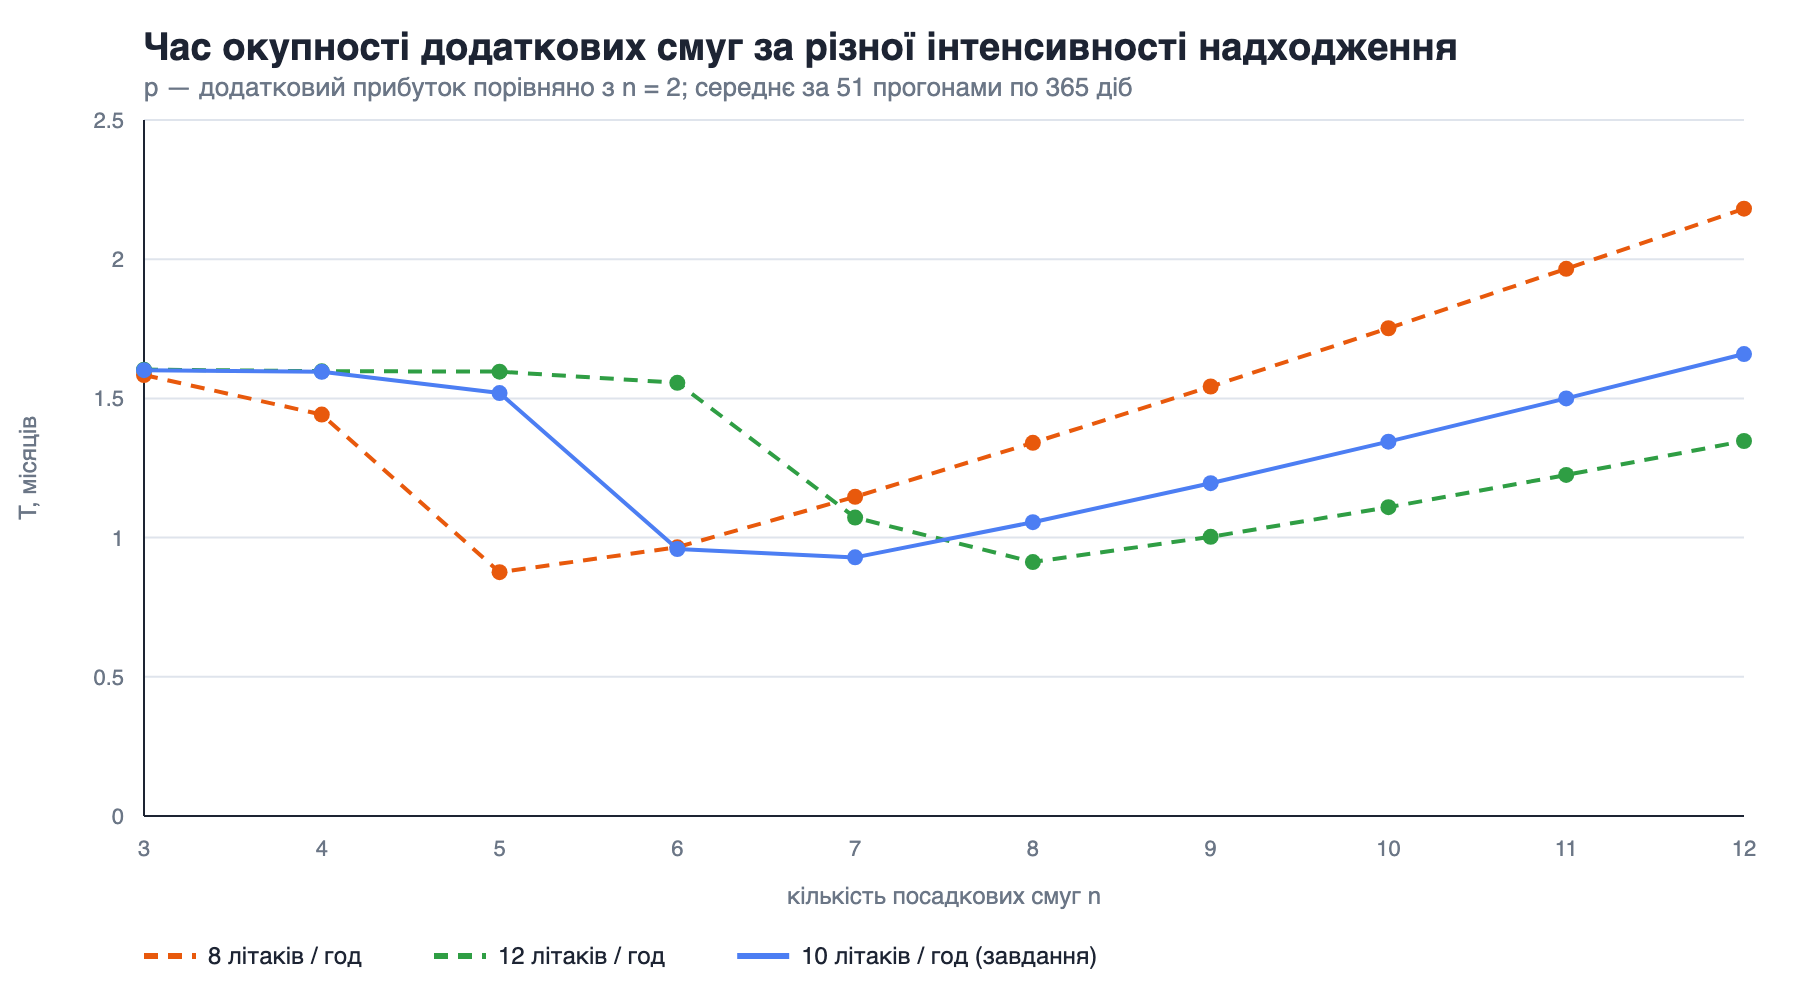
\includegraphics[width=0.92\textwidth]{sensitivity.png}
\caption{Час окупності додаткових смуг за різної інтенсивності надходження літаків}
\label{fig:sensitivity}
\end{figure}

Оптимальна кількість смуг залежить від потоку. За 8~літаків на годину найкраще мати 5~смуг ($T_{\Delta} = 0{,}876$~міс.), за 12~літаків -- 8~смуг ($T_{\Delta} = 0{,}912$~міс.). Закономірність та сама, що й для заданого потоку: потрібне середнє навантаження становить $\lambda \cdot t_s$, тобто 4,67, 5,83 і 7,0~смуги, і оптимум -- найменша кількість смуг, що з запасом перевищує це навантаження. Кількість смуг, рівна навантаженню з запасом менше 0,2~смуги (6~смуг за 10~літаків на годину), гірша: черга ще накопичується в години піків, і частина літаків дозаправляється.

Рекомендація чутлива до похибок у потоці, але помилка в бік більшої кількості смуг коштує мало. Якщо збудувати 5~додаткових смуг, а потік виявиться 12~літаків на годину, окупність становитиме 1,07~міс. замість найкращих 0,91. Якщо ж збудувати 6~додаткових смуг за заданого потоку, окупність становитиме 1,06~міс. замість 0,93. Натомість нестача смуг обходиться дорого: за 12~літаків на годину і 6~смугах прибуток лише 32,5~млн~грн на рік проти 107,9 за 7~смуг.

Отже, за заданої інтенсивності 10~літаків на годину слід будувати 5~додаткових смуг. Якщо аеропорт очікує зростання потоку, доцільно передбачити місце для шостої додаткової смуги й збудувати її, коли інтенсивність наблизиться до 12~літаків на годину.

\subsection{Висновки до розділу}

Двох смуг недостатньо для потоку 10~літаків на годину, тому аеропорт збитковий через масові дозаправки й відльоти. Найкоротша окупність, 0,93~міс., досягається за п'яти додаткових смуг, що й пропонується збудувати: це дає прибуток 151,2~млн~грн на рік, усуває відльоти і скорочує очікування до 8,8~хв. Пробний запуск за 8 і 12~літаків на годину показав, що оптимальна кількість смуг -- найменша, яка з запасом перевищує середнє навантаження $\lambda \cdot t_s$, і що за зростання потоку до 12~літаків на годину варто додати шосту смугу.

\structural{ВИСНОВКИ}

У роботі побудовано імітаційну модель системи посадки літаків в аеропорту на основі формального опису стохастичною мережею Петрі та визначено кількість посадкових смуг, за якої час окупності додаткових смуг мінімальний.

Концептуальна модель виділяє потік літаків, посадкові смуги, чергу очікування і фінансову підсистему. Формальний опис -- мережа Петрі з 13~позицій і 10~переходів. Головна складність задачі -- індивідуальні таймери дозаправки й відльоту кожного літака. У звичайній мережі Петрі маркери безіменні, і таймер одного літака забирав би з черги інший. Тому мережу доповнено маркерами-об'єктами та дугами, що беруть маркери одного об'єкта. Це невелике розширення формалізму зберегло модель компактною: кожен таймер -- це перехід із затримкою і пара переходів, що перевіряють, чи літак досі в черзі.

Алгоритм імітації реалізовано мовою TypeScript без бібліотек імітаційного моделювання. Він просуває час від події до події, підтримує багатоканальні переходи, інформаційні дуги та розв'язання конфліктів за пріоритетом і ймовірністю. Коректність алгоритму підтверджено модульними тестами, зокрема відтворенням теоретичних характеристик СМО M/M/1, а коректність моделі -- верифікацією на восьми наборах вхідних даних, де результати узгоджуються з формулою Літтла і граничними випадками.

Експериментальне дослідження проведено з прогонами тривалістю рік модельного часу після доби розгону, по 51~прогону для кожної кількості смуг, що забезпечує точність річного прибутку 1~млн~грн з довірчою ймовірністю 0,95. Результати такі:
\begin{itemize}
\item за двох смуг аеропорт збитковий ($-42{,}5$~млн~грн/рік): смуги перевантажені, майже кожен літак дозаправляється, а дві третини відлітають;
\item час окупності мінімальний за семи смуг, тобто за п'яти додаткових: 0,93~міс. за приростом прибутку і 1,19~міс. за загальним прибутком; витрати 15~млн~грн повертаються менш ніж за місяць;
\item за семи смуг жоден літак не відлітає, середнє очікування скорочується з 132 до 9~хв, а річний прибуток становить 151~млн~грн;
\item пробний запуск показав, що оптимум залежить від потоку: за 8~літаків на годину найкраще 5~смуг, за 12 -- 8~смуг; тому за очікуваного зростання потоку варто передбачити шосту додаткову смугу.
\end{itemize}

Прийняті припущення: пороги та грошові величини вигляду «$a \pm b$» розподілені рівномірно, літак дозаправляється не більше одного разу, черга обслуговується в порядку прибуття, у прибуток входять лише дохід від посадок і витрати на дозаправку. Не відтворено інших витрат аеропорту (утримання смуг, персонал), бо умова їх не задає; за їх наявності оптимальна кількість смуг може зменшитись.

Імітаційне моделювання виявилось доречним: воно врахувало нетерплячість літаків з двома порогами, випадкові доходи й витрати та дало оцінку точності результату, чого не дають формули теорії масового обслуговування. Моделювання вважаю успішним. Подальше дослідження варто спрямувати на зміну інтенсивності потоку протягом доби та на правила черги, наприклад пріоритет посадки літакам, що наближаються до порогу дозаправки.

% ДСТУ 8302:2015, у порядку першої згадки в тексті.
\begin{thebibliography}{9}
\bibitem{stetsenko2010} Стеценко І. В. Моделювання систем : навч. посіб. Черкаси : ЧДТУ, 2010. 399~с.
\bibitem{tomashevskyi2005} Томашевський В. М. Моделювання систем. Київ : Видавнича група BHV, 2005. 352~с.
\bibitem{stetsenko2024} Стеценко І. В., Дифучина О. Ю., Дифучин А. Ю. Моделювання систем. Курсова робота : рек. до виконання курсов. роботи : навч. посіб. Київ : КПІ ім. Ігоря Сікорського, 2024. 109~с.
\bibitem{jensen2009} Jensen K., Kristensen L. M. Coloured Petri Nets: Modelling and Validation of Concurrent Systems. Berlin ; Heidelberg : Springer, 2009. 384~p.
\bibitem{typescript} TypeScript Documentation. Microsoft. URL: \url{https://www.typescriptlang.org/docs/} (дата звернення: 13.11.2026).
\bibitem{bun} Bun Documentation. Oven. URL: \url{https://bun.sh/docs} (дата звернення: 13.11.2026).
\bibitem{kelton2024} Kelton W. D., Ivey N. B., Zupick N. Simulation with Arena. 7th ed. New York : McGraw-Hill, 2024. 611~p.
\bibitem{law2015} Law A. M. Simulation Modeling and Analysis. 5th ed. New York : McGraw-Hill Education, 2015. 804~p.
\end{thebibliography}

\appendices

\appendix[app:petri]{Лістинг алгоритму імітації мережі Петрі}
\tsfile{src/petri.ts}

\appendix[app:random]{Лістинг генераторів випадкових величин і статистичної обробки}
\tsfile{src/random.ts}
\tsfile{src/stats.ts}

\appendix[app:airport]{Лістинг моделі аеропорту}
\tsfile{src/airport.ts}

\appendix[app:experiments]{Лістинг проведення експериментів}
\tsfile{src/experiments.ts}
\tsfile{src/index.ts}

\end{document}
